\documentclass[a4paper]{article}
\usepackage{graphicx}
\usepackage{amsmath}
\usepackage{amsthm}
\usepackage{listings}
\usepackage{xcolor}
\usepackage{geometry}
\usepackage{booktabs}
\usepackage{float}
\usepackage{subcaption}

\newgeometry{margin=1in}

\lstset{language=Octave, basicstyle=\ttfamily\small,
        keywords={for, if, else, endif, endfor, ones, zeros},
        keywordstyle=\color{purple}, commentstyle=\color{gray}, stringstyle=\color{blue}}

\renewcommand{\thesubsection}{\thesection.\Alph{subsection}}


\begin{document}
    \begin{center}
        \vspace*{-0.5in}
        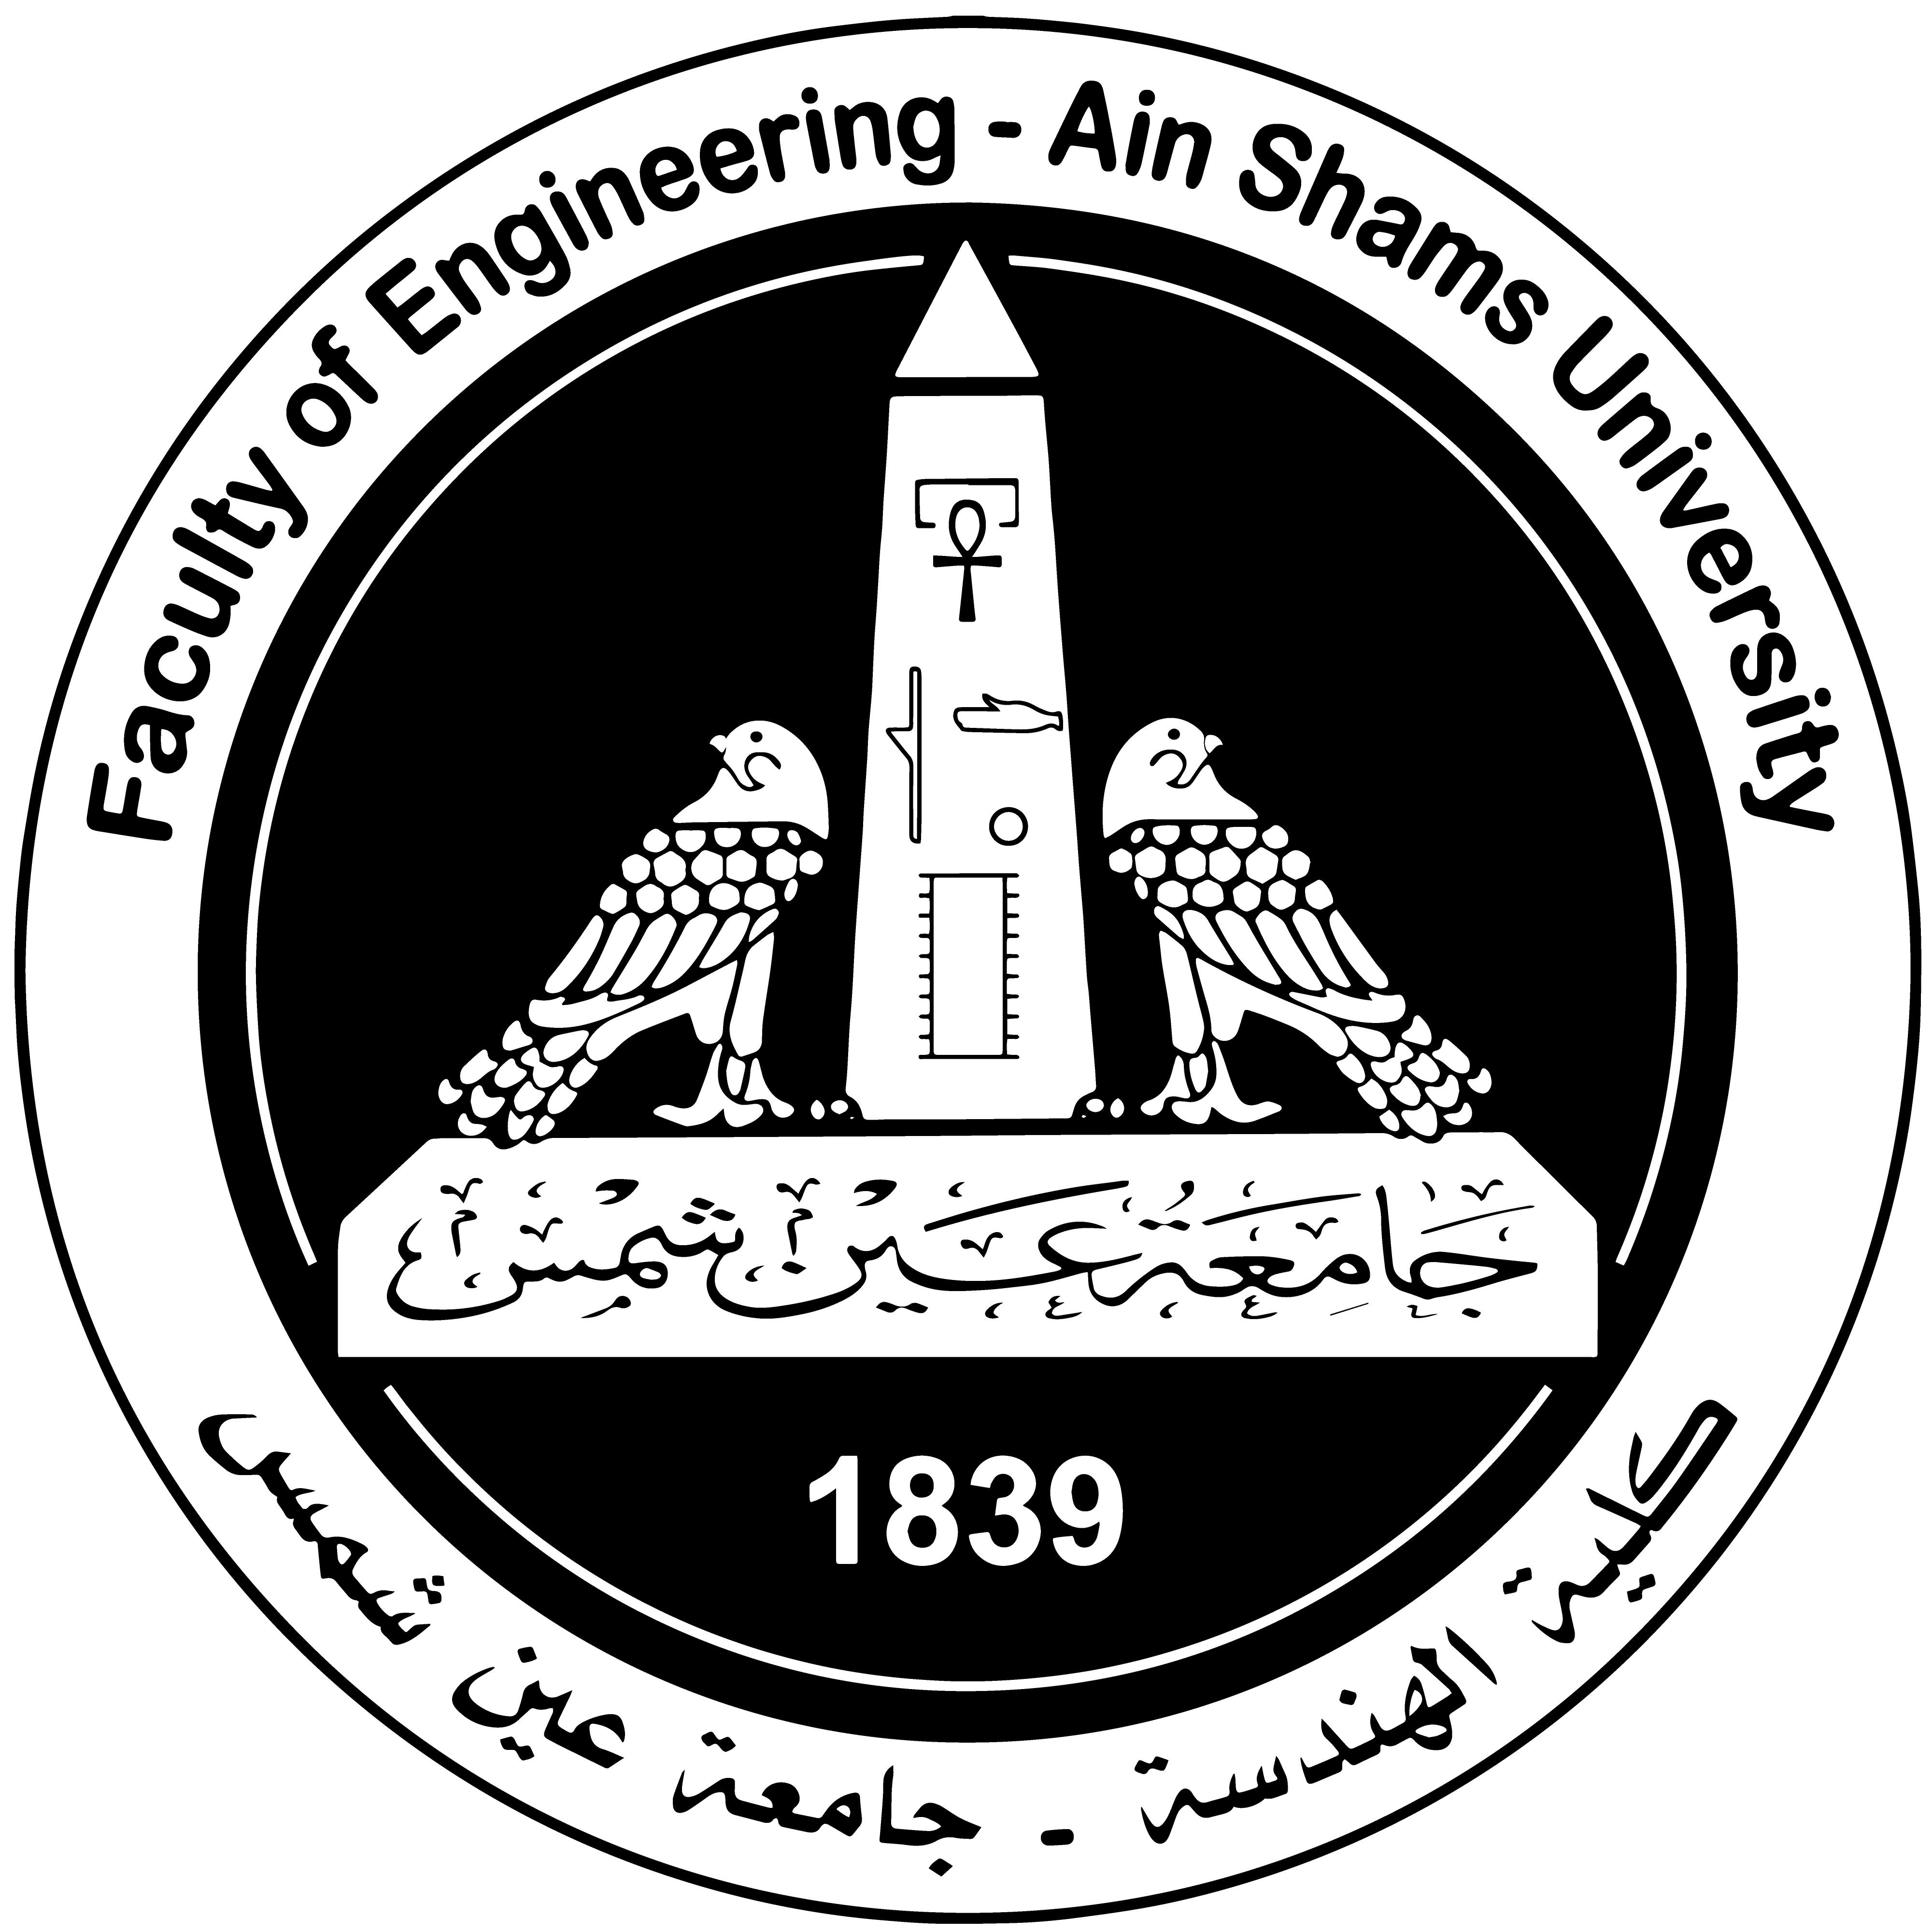
\includegraphics[width=100pt]{180207 ASU-Logo-Black-4000.png}
        \\ \vspace{15pt}
        \textbf{\huge Communication Systems Project Report}
        \\ \vspace{30pt}
        \Large Ain Shams University \\ Faculty of Engineering
        \\ \vspace{15pt}
        \textbf{Under the Supervision of}
        \\
        \textit{\Large Dr. Mazen Erfan}\\
        \textit{\Large Dr. Alaa El-Deen Fathy}
        \\[1.5cm]
        \textbf{\Large Team Members}
        \\[0.5cm]
        \begin{tabular}{c c c c c}
            \textbf{Name} & \textbf{Code} & \textbf{Dept.} & \textbf{Sec.} & \textbf{Contributions} \\[5pt]
            \hline \\[-10pt]
            \textit{\large \textbf{Farida Hatem Mostafa Reda}} & \textit{\large 2401395} & \large CSE & \textit{\large 3} & \\
            \textit{\large Habiba Ahmed Ebrahim} & \textit{\large 2401036} & \large CSE & \textit{\large 3} & \\
            \textit{\large Hana Hassan Sayed Hassan} & \textit{\large 2401266} & \large CSE & \textit{\large 3} & \\
            \textit{\large Amr Mohamed Ghonimy Kassab} & \textit{\large 2400531} & \large CSE & \textit{\large 3} & \\
            \textit{\large Mohamed Yehia Tawfik} & \textit{\large 2400646} & \large CSE & \textit{\large 3} & \\
            \textit{\large Eiad Salama Ahmed} & \textit{\large 2400098} & \large CSE & \textit{\large 3} & \\
            \textit{\large Ziad Tarek Fouad} & \textit{\large 2400429} & \large CSE & \textit{\large 3} & \textit{\large dig\_part\_c} \\
            \textit{\large Omar Ehab Mohamed Ali Almaz} & \textit{\large 2400621} & \large CSE & \textit{\large 3} & \\
            \textit{\large Moaaz Mostafa Ibrahim Ahmed} & \textit{\large 2400862} & \large ECE & \textit{\large 3} & \\
            \textit{\large Ahmed Gamal Roushdy} & \textit{\large 2400315} & \large ECE & \textit{\large 3} & \\
        \end{tabular}
    \end{center}
\pagebreak

\section{Analog Communication}
\subsection{Part A: Amplitude Modulation}

\subsubsection{Item 5: Double Sideband - Suppressed Carrier (DSB-SC) Modulation}

\paragraph{Theoretical Derivation and Spectral Analysis.}
The baseband message signal $m(t)$ is defined over a 5-second interval as:
\begin{equation}
m(t) = \begin{cases} \cos(2\pi f_m t), & 0 \le t < 5\text{ s} \\ 0, & \text{otherwise} \end{cases}
\end{equation}
where $f_m = 20\text{ Hz}$. The high-frequency sinusoidal carrier signal is given by $c(t) = \cos(2\pi f_c t)$ with $f_c = 200\text{ Hz}$.

The DSB-SC modulated waveform $s_{\text{DSB}}(t)$ is produced by multiplying the message signal directly by the carrier:
\begin{equation}
s_{\text{DSB}}(t) = m(t) \cdot c(t) = \cos(2\pi f_m t) \cos(2\pi f_c t)
\end{equation}
Applying the trigonometric product identity yields:
\begin{equation}
s_{\text{DSB}}(t) = \frac{1}{2} \cos\left(2\pi (f_c - f_m) t\right) + \frac{1}{2} \cos\left(2\pi (f_c + f_m) t\right)
\end{equation}

Taking the Fourier Transform of $s_{\text{DSB}}(t)$:
\begin{equation}
S_{\text{DSB}}(f) = \frac{1}{2} \left[ M(f - f_c) + M(f + f_c) \right]
\end{equation}

The spectrum consists of two discrete sidebands symmetric about the origin:
\begin{itemize}
    \item \textbf{Upper Sideband (USB):} Located at $\pm (f_c + f_m) = \pm 220\text{ Hz}$ with spectral magnitude $0.25$.
    \item \textbf{Lower Sideband (LSB):} Located at $\pm (f_c - f_m) = \pm 180\text{ Hz}$ with spectral magnitude $0.25$.
    \item \textbf{Carrier Component:} At $f = \pm f_c = \pm 200\text{ Hz}$, the spectrum magnitude is zero, confirming carrier suppression.
\end{itemize}

Using the 1\% maximum spectral magnitude threshold criterion, the theoretical bandwidth is:
\begin{equation}
B_{\text{DSB-SC}} = 2 f_m = 2 \times 20\text{ Hz} = 40\text{ Hz}
\end{equation}

\begin{figure}[H]
    \centering
    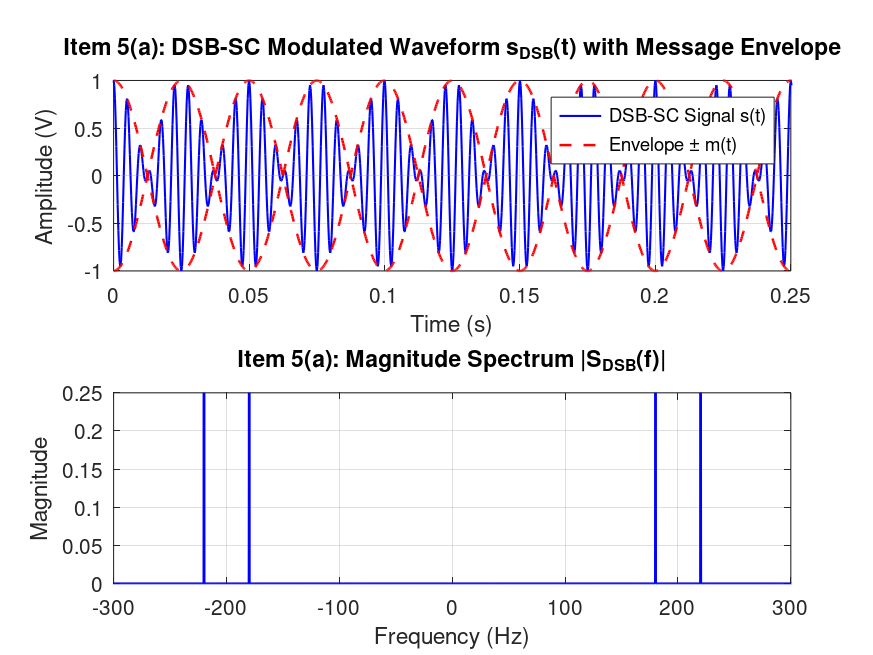
\includegraphics[width=0.85\textwidth]{Octave Scripts/Analog_PA_I5abc_Figs/Item5(a).png}
    \caption{Item 5(a): Time-domain DSB-SC modulated waveform $s_{\text{DSB}}(t)$ with message envelope overlay (top) and magnitude spectrum $|S_{\text{DSB}}(f)|$ displaying carrier suppression (bottom).}
    \label{fig:dsbsc_signal}
\end{figure}

\paragraph{Coherent Demodulation.}
Coherent detection requires multiplying $s_{\text{DSB}}(t)$ at the receiver by a local oscillator matched perfectly in frequency and phase ($2\cos(2\pi f_c t)$):
\begin{equation}
v(t) = s_{\text{DSB}}(t) \cdot \left[2 \cos(2\pi f_c t)\right] = 2 m(t) \cos^2(2\pi f_c t)
\end{equation}
Using $\cos^2(\theta) = \frac{1 + \cos(2\theta)}{2}$:
\begin{equation}
v(t) = m(t) \left[1 + \cos(4\pi f_c t)\right] = \underbrace{m(t)}_{\text{Baseband Message}} + \underbrace{m(t) \cos(4\pi f_c t)}_{\text{High-Frequency Component at } 2f_c = 400\text{ Hz}}
\end{equation}

Passing $v(t)$ through a frequency-domain Low-Pass Filter (LPF) with cutoff frequency $W = 30\text{ Hz}$ eliminates the $400\text{ Hz}$ component, yielding complete message recovery:
\begin{equation}
\hat{m}(t) = \text{LPF}\{v(t)\} = m(t)
\end{equation}

\begin{figure}[H]
    \centering
    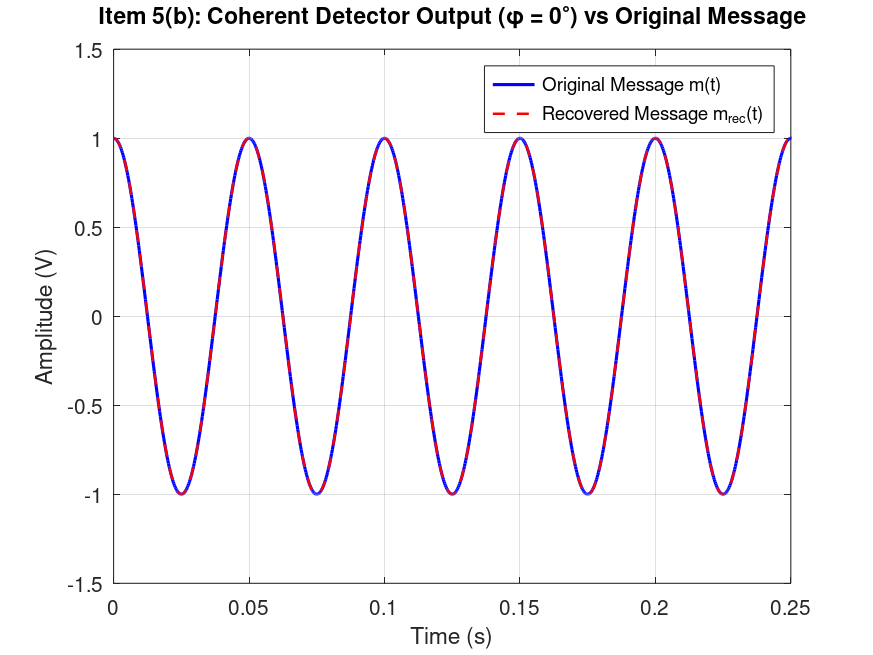
\includegraphics[width=0.8\textwidth]{Octave Scripts/Analog_PA_I5abc_Figs/Item5(b).png}
    \caption{Item 5(b): Coherent detector output ($\phi = 0^\circ$) overlaid on the original message $m(t)$.}
    \label{fig:coherent_ideal}
\end{figure}

\paragraph{Effect of Local Oscillator Phase Error.}
If the local oscillator has a phase error $\phi$, such that $c_{\text{local}}(t) = 2 \cos(2\pi f_c t + \phi)$, the product signal becomes:
\begin{equation}
v_\phi(t) = 2 m(t) \cos(2\pi f_c t) \cos(2\pi f_c t + \phi) = m(t) \left[ \cos(\phi) + \cos(4\pi f_c t + \phi) \right]
\end{equation}

After low-pass filtering:
\begin{equation}
\hat{m}_\phi(t) = m(t) \cos(\phi)
\end{equation}

The recovered amplitude scales with $\cos(\phi)$:
\begin{itemize}
    \item \textbf{For $\phi = 30^\circ$:} $\hat{m}(t) = m(t) \cos(30^\circ) = 0.866\, m(t)$ ($13.4\%$ amplitude reduction).
    \item \textbf{For $\phi = 60^\circ$:} $\hat{m}(t) = m(t) \cos(60^\circ) = 0.500\, m(t)$ ($50.0\%$ amplitude reduction).
    \item \textbf{For $\phi = 90^\circ$:} $\hat{m}(t) = m(t) \cos(90^\circ) = 0$ (\textbf{Quadrature Null Effect}).
\end{itemize}

\begin{figure}[H]
    \centering
    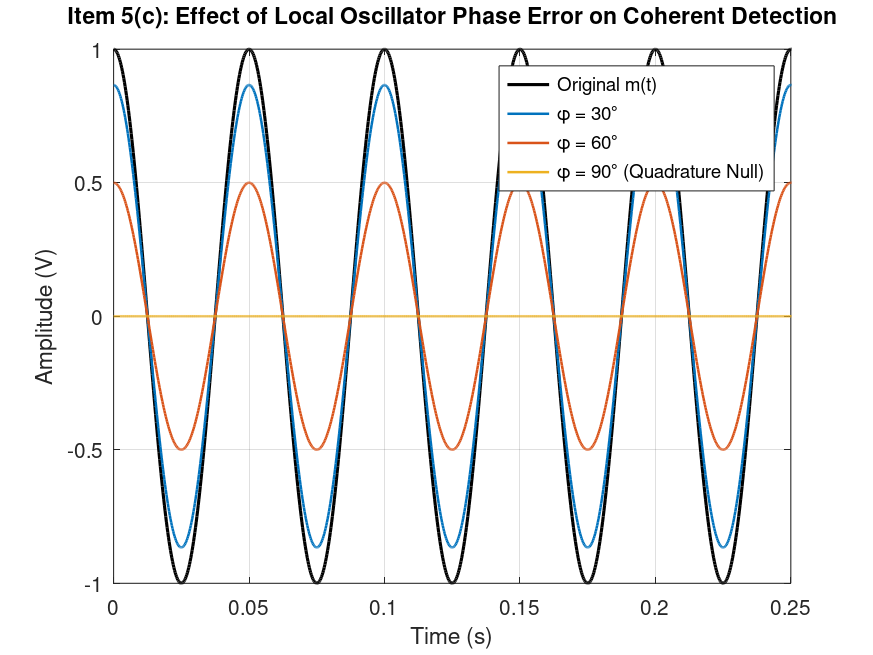
\includegraphics[width=0.8\textwidth]{Octave Scripts/Analog_PA_I5abc_Figs/Item5(c).png}
    \caption{Item 5(c): Demodulated signal degradation across local oscillator phase errors $\phi \in \{30^\circ, 60^\circ, 90^\circ\}$.}
    \label{fig:phase_errors}
\end{figure}

\subsubsection{Item 7: Conventional Amplitude Modulation (AM) and Envelope Detector}

\paragraph{Conventional AM Modulation ($k_a = 0.4$).}
Conventional AM is generated by adding a DC carrier component prior to modulation:
\begin{equation}
s_{\text{AM}}(t) = A_c \left[ 1 + k_a m(t) \right] \cos(2\pi f_c t)
\end{equation}
For $A_c = 1$, $k_a = 0.4$, and $m(t) = \cos(2\pi \cdot 20 \cdot t)$:
\begin{equation}
s_{\text{AM}}(t) = \left[ 1 + 0.4 \cos(2\pi \cdot 20 \cdot t) \right] \cos(2\pi \cdot 200 \cdot t)
\end{equation}
The modulation index is $\mu = k_a \cdot \max|m(t)| = 0.4$ ($40\%$ modulation).

The spectrum contains a discrete carrier component at $\pm 200\text{ Hz}$ of magnitude $0.5$, and two sidebands at $\pm 180\text{ Hz}$ and $\pm 220\text{ Hz}$ of magnitude $0.1$. The bandwidth remains $B_{\text{AM}} = 2 f_m = 40\text{ Hz}$.

\paragraph{Envelope Detector Performance and Choice of $RC$.}
Demodulation is performed using a diode-capacitor envelope detector governed by the discrete charging and discharging update equations. To avoid carrier ripple and diagonal clipping, $RC$ must satisfy:
\begin{equation}
\frac{1}{f_c} \ll RC \ll \frac{1}{f_m} \implies 0.005\text{ s} \ll RC \ll 0.050\text{ s}
\end{equation}
Furthermore, the non-clipping constraint is given by:
\begin{equation}
RC \le \frac{\sqrt{1 - \mu^2}}{2\pi f_m \mu} = \frac{\sqrt{1 - 0.4^2}}{2\pi \times 20 \times 0.4} \approx 0.0182\text{ s}
\end{equation}

Selecting $RC_{\text{opt}} = 0.015\text{ s}$ satisfies all bounds. The performance of three distinct $RC$ values is evaluated:
\begin{itemize}
    \item $RC = 0.001\text{ s}$ ($RC \ll 1/f_c$): Discharges too rapidly between carrier peaks, introducing excessive high-frequency carrier ripple.
    \item $RC = 0.015\text{ s}$ (Optimal): Discharges at a rate matching the maximum downward slope of the message envelope.
    \item $RC = 0.100\text{ s}$ ($RC > \text{bound}$): Discharges too slowly, failing to follow the falling envelope and causing \textbf{diagonal clipping}.
\end{itemize}

\begin{figure}[H]
    \centering
    \begin{subfigure}[b]{0.48\textwidth}
        \centering
        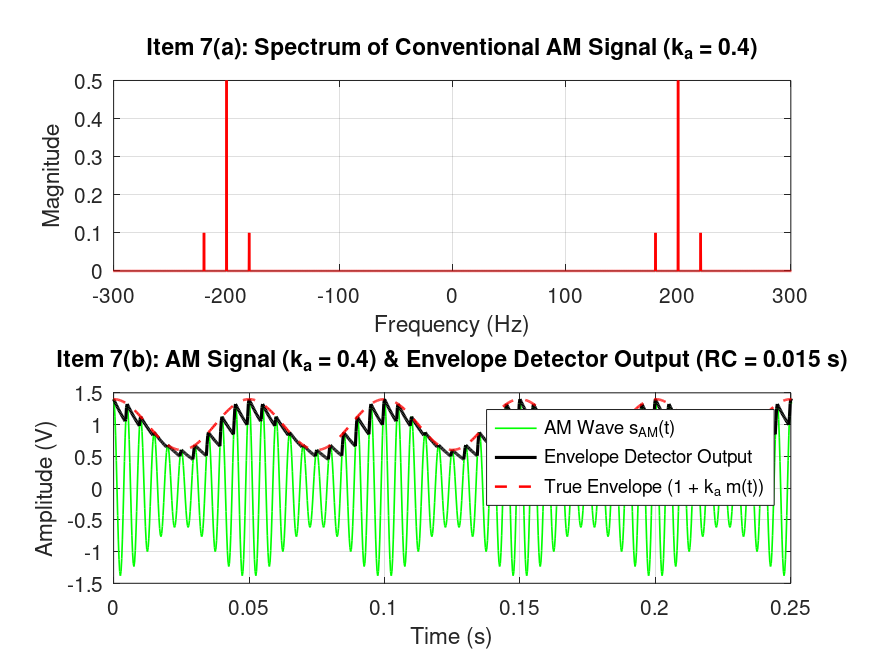
\includegraphics[width=\textwidth]{Octave Scripts/Analog_PA_I7abc_Figs/Item7(a)(b).png}
        \caption{Spectrum and Optimal Envelope Detection ($k_a = 0.4$, $RC = 0.015\text{ s}$)}
    \end{subfigure}
    \hfill
    \begin{subfigure}[b]{0.48\textwidth}
        \centering
        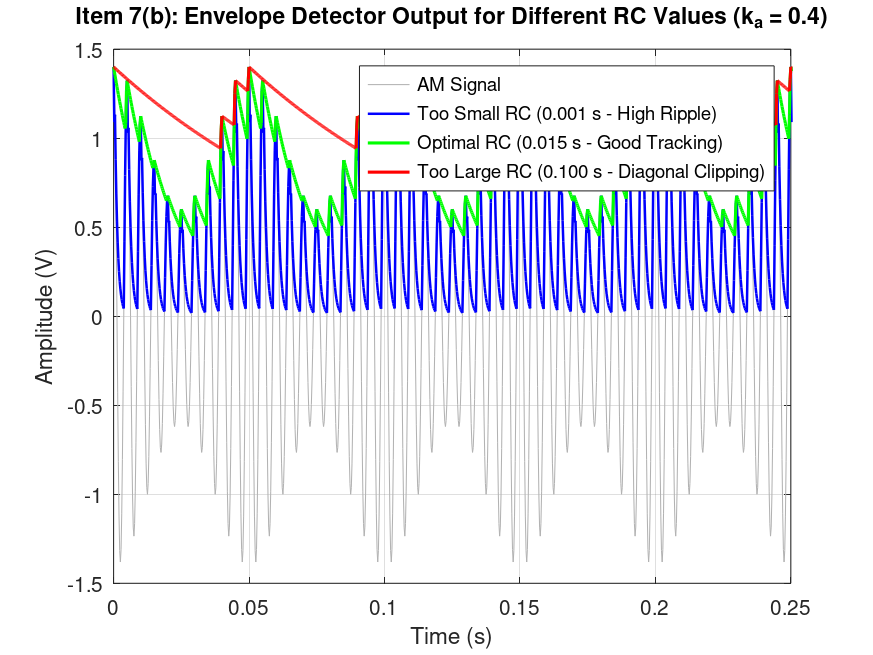
\includegraphics[width=\textwidth]{Octave Scripts/Analog_PA_I7abc_Figs/Item7(b).png}
        \caption{Envelope Detector Output vs.\ $RC$}
    \end{subfigure}
    \caption{Item 7(a \& b): Conventional AM spectrum, modulated signal, and envelope detector tracking across different $RC$ relaxation time constants.}
    \label{fig:am_ka04}
\end{figure}

\paragraph{Over-Modulation Analysis ($k_a = 1.5$).}
When the amplitude sensitivity is increased to $k_a = 1.5$, the modulation index becomes $\mu = 1.5 > 1.0$ ($150\%$ modulation).

When $m(t) < -1/1.5 = -0.667$, the envelope term $(1 + 1.5\, m(t))$ becomes negative, causing a $180^\circ$ carrier phase reversal and envelope crossovers. Because a non-coherent envelope detector tracks the absolute envelope magnitude $|1 + 1.5\, m(t)|$, the negative portion of the envelope is rectified upward, producing severe non-linear harmonic distortion in the recovered message.

\begin{figure}[H]
    \centering
    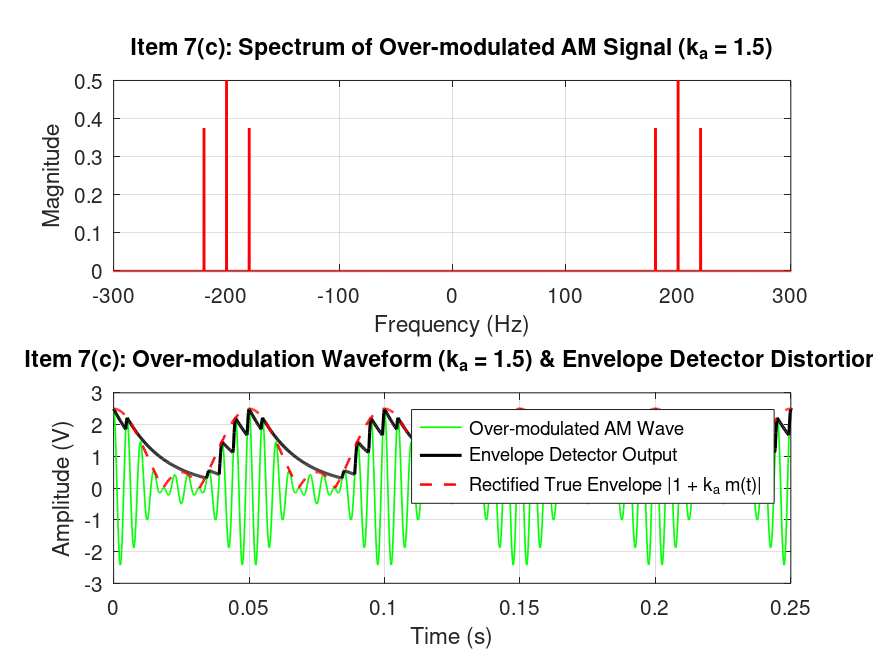
\includegraphics[width=0.85\textwidth]{Octave Scripts/Analog_PA_I7abc_Figs/Item7(c).png}
    \caption{Item 7(c): Over-modulated AM spectrum ($k_a = 1.5$, top) and waveform with envelope detector output demonstrating severe rectification distortion (bottom).}
    \label{fig:overmodulation}
\end{figure}

\subsubsection{Summary of Results}

Table~\ref{tab:results_summary} summarizes all theoretical and simulated metrics obtained for Part A (Items 5 \& 7).

\begin{table}[H]
\centering
\caption{Consolidated Numerical Results for Analog AM Systems}
\label{tab:results_summary}
\begin{tabular}{l c c c}
\toprule
\textbf{Parameter / Metric} & \textbf{DSB-SC} & \textbf{AM ($k_a = 0.4$)} & \textbf{AM ($k_a = 1.5$)} \\
\midrule
Carrier Frequency ($f_c$) & $200\text{ Hz}$ & $200\text{ Hz}$ & $200\text{ Hz}$ \\
Message Frequency ($f_m$) & $20\text{ Hz}$ & $20\text{ Hz}$ & $20\text{ Hz}$ \\
Modulation Index ($\mu$) & N/A & $0.40$ & $1.50$ \\
Theoretical Bandwidth & $40.00\text{ Hz}$ & $40.00\text{ Hz}$ & $40.00\text{ Hz}$ \\
Simulated Bandwidth (1\% threshold) & $40.00\text{ Hz}$ & $40.00\text{ Hz}$ & $40.00\text{ Hz}$ \\
Carrier Spectrum Magnitude & $0.000$ & $0.500$ & $0.500$ \\
Sideband Spectrum Magnitude & $0.250$ & $0.100$ & $0.375$ \\
Demodulator Scheme & Coherent Filter & Envelope Detector & Envelope Detector \\
Optimal Receiver Parameter & $W = 30\text{ Hz}$ & $RC = 0.015\text{ s}$ & $RC = 0.015\text{ s}$ \\
Demodulation Quality & Perfect ($\phi = 0^\circ$) & Distortion-free & Severe Distortion \\
\bottomrule
\end{tabular}
\end{table}


\section{Digital Communication}
\subsection{Sampling, Quantization, and PCM}
\subsubsection{Sampling}
\newcommand{\samplingfig}[2]{\par\medskip\noindent\begin{minipage}{\textwidth}\centering
\includegraphics[width=0.95\textwidth]{#1}\par\smallskip
\refstepcounter{figure}Figure \thefigure: #2\end{minipage}\par\medskip}
The message is $m(t)=\cos(2\pi 20t)+0.5\cos(2\pi 50t)$, so its bandwidth is $W=50$ Hz and the Nyquist rate is $f_N=2W=100$ Hz. Ideal sampling is modelled as multiplication by an impulse train, which gives $M_s(f)=f_s\sum_k M(f-kf_s)$: copies of $M(f)$ centred at multiples of $f_s$. The simulation uses a fine grid of 16000 Hz over a 1 s window, so every sampling rate used is an exact whole number of grid points. The sampler, the ideal low-pass filter (LPF), the pulse train and the equalizer are all written by hand, with no toolbox functions.
\samplingfig{Octave Scripts/digA_items1to3_figures/00_message.png}{The message $m(t)$ and its spectrum: lines at $\pm20$ Hz (0.5) and $\pm50$ Hz (0.25).}

\paragraph{Item 1: sampling at $f_N$ and at $4f_N$.}
At $f_s=100$ Hz and $f_s=400$ Hz we sampled $m(t)$ and recovered it with an ideal LPF of cutoff $f_s/2$. In both cases the maximum error between the recovered signal and $m(t)$ is about $10^{-14}$ V, so the signal is recovered exactly. A second LPF, a Hamming-windowed sinc FIR filter built with \texttt{conv}, was used as an independent check.

\samplingfig{Octave Scripts/digA_items1to3_figures/01_item1_fs100.png}{Sampling at $f_s=100$ Hz (Nyquist rate): samples, spectrum and reconstruction.}
\samplingfig{Octave Scripts/digA_items1to3_figures/01_item1_fs400.png}{Sampling at $f_s=400$ Hz ($4\times$ Nyquist): the copies of $M(f)$ are well separated.}

At exactly the Nyquist rate the 50 Hz line of the base-band copy and of the neighbouring copy fall on the same frequency, which is also the LPF edge. The recovered 50 Hz amplitude then depends on the gain the ``ideal'' filter takes at its edge: with edge gain 1, 1/2 and 0 the recovered amplitude is 1, 0.5 and 0 (the true value is 0.5). Only the value 1/2 recovers the signal. For $\sin(2\pi 50t)$ sampled at 100 Hz, every sample is zero, so that signal is lost completely. This is why a signal should be sampled strictly above $2W$.

\samplingfig{Octave Scripts/digA_items1to3_figures/02_item1_nyquist_edge.png}{Effect of the LPF gain at exactly 50 Hz when $f_s=100$ Hz.}

\paragraph{Item 2: sampling below the Nyquist rate.}
At $f_s=80$ Hz the 20 Hz tone is still sampled legally ($80>2\cdot 20$), but the 50 Hz tone is not. A tone at $f_0$ reappears at $|f_0-kf_s|$, so 50 Hz folds to $|50-80|=30$ Hz. After the best possible LPF ($f_c=40$ Hz) the output contains lines at 20 Hz and 30 Hz and none at 50 Hz. The output matches $\cos(2\pi 20t)+0.5\cos(2\pi 30t)$ to about $10^{-14}$ V, and its RMS error against the original is 0.500 V. Once aliasing has happened, the original cannot be recovered by filtering.

\samplingfig{Octave Scripts/digA_items1to3_figures/03_item2_aliasing.png}{Aliasing at $f_s=80$ Hz: overlapping copies and the reconstructed signal.}

\paragraph{Item 3: natural and flat-top sampling.}
Both use $f_s=400$ Hz ($T_s=2.5$ ms) and a duty cycle of 25\%, so the pulse width is $\tau=0.625$ ms. Natural sampling multiplies $m(t)$ by a periodic pulse train $p(t)$, so the pulse tops follow $m(t)$. Flat-top sampling reads $m(t)$ only at the sampling instant and holds it for $\tau$. The spectrum of the flat-top signal is multiplied by $\operatorname{sinc}(f\tau)$ (the aperture effect), while the natural-sampled copies are only scaled by a constant.

Natural samples are recovered with an LPF of gain $1/d$, where $d=0.25$. Flat-top samples are recovered with the same filter plus an equalizer $1/\operatorname{sinc}(f\tau)$ and a delay correction of $\tau/2$. At the band edge, $\operatorname{sinc}(50\tau)=0.99839$, which is a droop of 0.0140 dB (0.16\%), and $\operatorname{sinc}(20\tau)=0.99974$. The equalizer therefore needs only about $+0.014$ dB at 50 Hz. The effect is small because $\tau$ is much shorter than $T_s$.

\samplingfig{Octave Scripts/digA_items1to3_figures/04_item3_time.png}{Natural and flat-top sampled signals overlaid on the same axes together with $m(t)$ ($f_s=400$ Hz, 25\% duty): natural pulse tops follow $m(t)$, flat-top tops are constant.}
\samplingfig{Octave Scripts/digA_items1to3_figures/05_item3_spectra.png}{Spectra of natural and flat-top sampling overlaid on the same axes with the $\operatorname{sinc}(f\tau)$ envelope: natural copies are constant-scaled, flat-top copies are multiplied by $\operatorname{sinc}(f\tau)$.}
\samplingfig{Octave Scripts/digA_items1to3_figures/06_item3_recovery.png}{Recovery from natural and flat-top samples, recovery error, and aperture droop against equalizer gain.}

\begin{lstlisting}
fs = 400; N = fsim/fs;  d = 0.25;  w = round(d*N);
p      = double(mod(0:L-1,N) < w);      % pulse train
m_nat  = m .* p;                        % natural sampling
m_flat = zeros(size(m));
for n = 0:fs*T-1
  m_flat(n*N+1 : n*N+w) = m(n*N+1);     % hold the sample for tau
end
\end{lstlisting}

% =====================================================================
% Digital Part A, Items 4 & 5 -- Quantization and PCM
% =====================================================================
\subsubsection{Quantization (Item 4)}

\paragraph{Signal Dynamic Range (Asymmetric Message).}
For $m(t) = \cos(2\pi \cdot 20t) + 0.5\cos(2\pi \cdot 50t)$ ($W = 50\text{ Hz}$, fundamental frequency $f_0 = \gcd(20,50) = 10\text{ Hz}$, period $T_0 = 0.1\text{ s}$), the average message power is $P_{\text{sig}} = \frac{1^2}{2} + \frac{0.5^2}{2} = 0.6250\text{ W}$. Sampling at four times the Nyquist rate ($f_s = 400\text{ Hz}$, $T_s = 2.5\text{ ms}$) produces $N_s = 400$ samples over $1\text{ s}$. Evaluating $m(t)$ over a finely resolved period shows that the waveform is \textbf{asymmetric}: both cosine components peak positively together at $t = 0$ giving $V_{\max} = +1.5000\text{ V}$, whereas destructive alignment yields a minimum of $V_{\min} = -1.3529\text{ V}$ (rather than $-1.5\text{ V}$). Thus, the true dynamic range spanned by the quantizer is:
\begin{equation}
R = V_{\max} - V_{\min} = 1.5000 - (-1.3529) = 2.8529\text{ V}
\end{equation}

\begin{figure}[H]
    \centering
    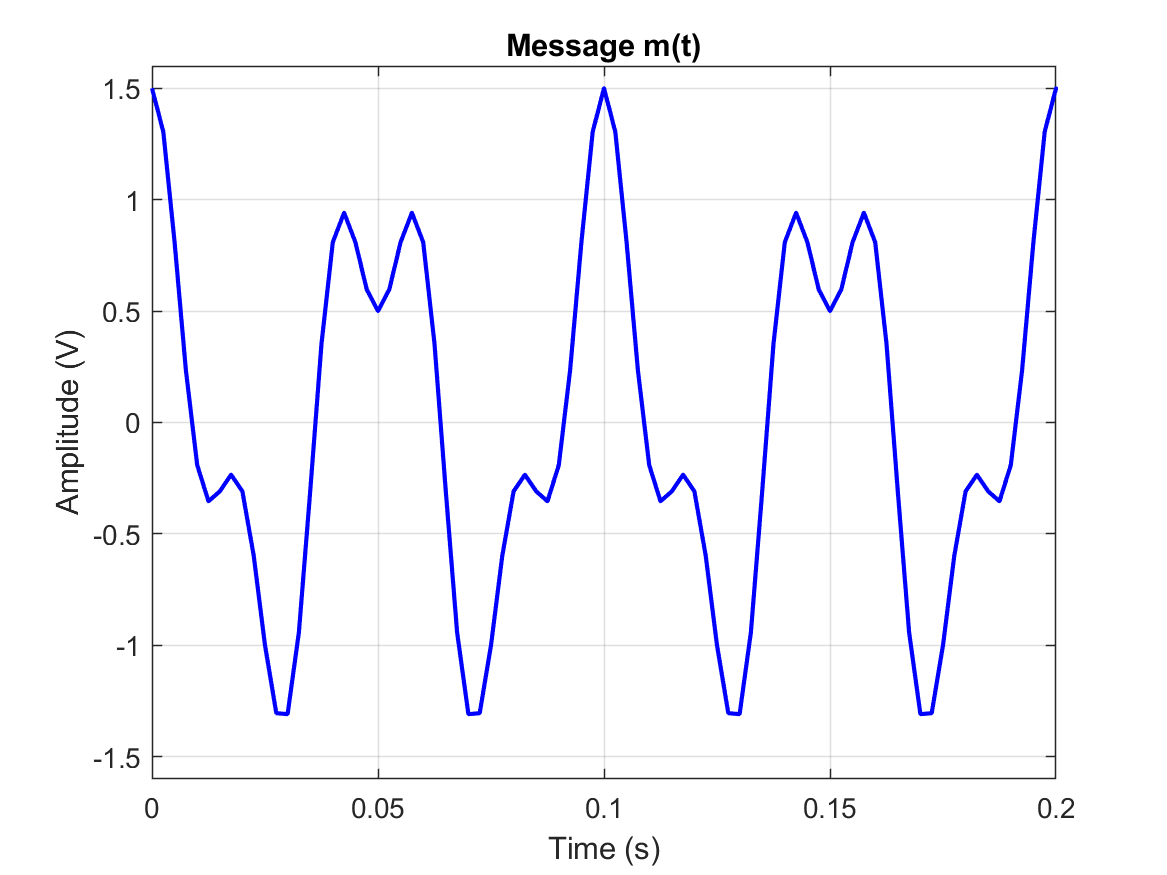
\includegraphics[width=0.72\textwidth]{Octave Scripts/digA_item4_5_figures/Message_m_t.png}
    \caption{Sampled message signal $m(t)$ over two fundamental periods ($0.2\text{ s}$), illustrating its asymmetric amplitude swing between $V_{\min} = -1.3529\text{ V}$ and $V_{\max} = +1.5000\text{ V}$.}
    \label{fig:digA_item4_msg}
\end{figure}

\paragraph{Item 4(a): Custom Mid-Tread and Mid-Rise Uniform Quantizers.}
For an $n$-bit uniform quantizer with $L = 2^n$ levels written directly from basic mathematical operations:
\begin{itemize}
    \item \textbf{Mid-Rise Quantizer:} Zero acts as a decision threshold rather than an output level. Dividing $[V_{\min}, V_{\max}]$ into $L$ equal cells gives step size $\Delta_{\text{rise}} = R / L$, cell index $k_{\text{rise}} = \min(\max(\lfloor (m - V_{\min})/\Delta_{\text{rise}} \rfloor, 0), L-1)$, and cell-center levels:
    \begin{equation}
    m_{q,\text{rise}} = V_{\min} + \left(k_{\text{rise}} + 0.5\right)\Delta_{\text{rise}}
    \end{equation}
    \item \textbf{Mid-Tread Quantizer:} Zero is explicitly included among the $L$ reconstruction levels ($m_q = k\,\Delta_{\text{tread}}$ for integer $k$). Because $L$ levels span $R$ across $L - 1$ steps without peak overload, the step size is $\Delta_{\text{tread}} = R / (L - 1)$, with $k_{\min} = \operatorname{round}(V_{\min}/\Delta_{\text{tread}})$, clamped index $k_{\text{tread}} = \min(\max(\operatorname{round}(m/\Delta_{\text{tread}}), k_{\min}), k_{\min}+L-1)$, and output:
    \begin{equation}
    m_{q,\text{tread}} = k_{\text{tread}}\,\Delta_{\text{tread}}
    \end{equation}
\end{itemize}

Figure~\ref{fig:digA_item4_errors} displays the quantization error $e(t) = m(t) - m_q(t)$ for both quantizers at $n = 3, 4, 6,$ and $8$ bits together with their respective $\pm\Delta/2$ bounds. Each additional bit doubles $L$ and halves the step size and error swing.

\begin{figure}[H]
    \centering
    \begin{subfigure}[b]{0.48\textwidth}
        \centering
        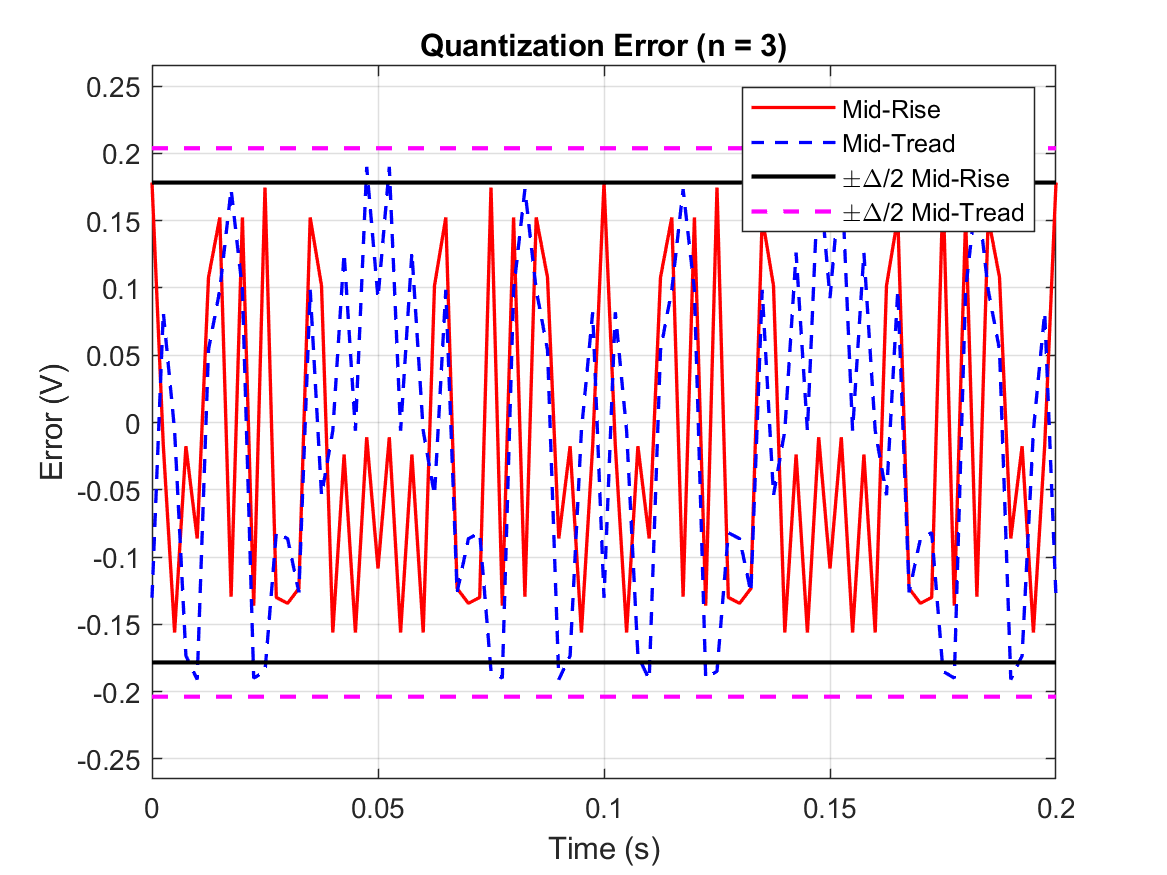
\includegraphics[width=\textwidth]{Octave Scripts/digA_item4_5_figures/Quantization_Error_n_3.png}
        \caption{$n = 3$ bits ($L = 8$)}
    \end{subfigure}\hfill
    \begin{subfigure}[b]{0.48\textwidth}
        \centering
        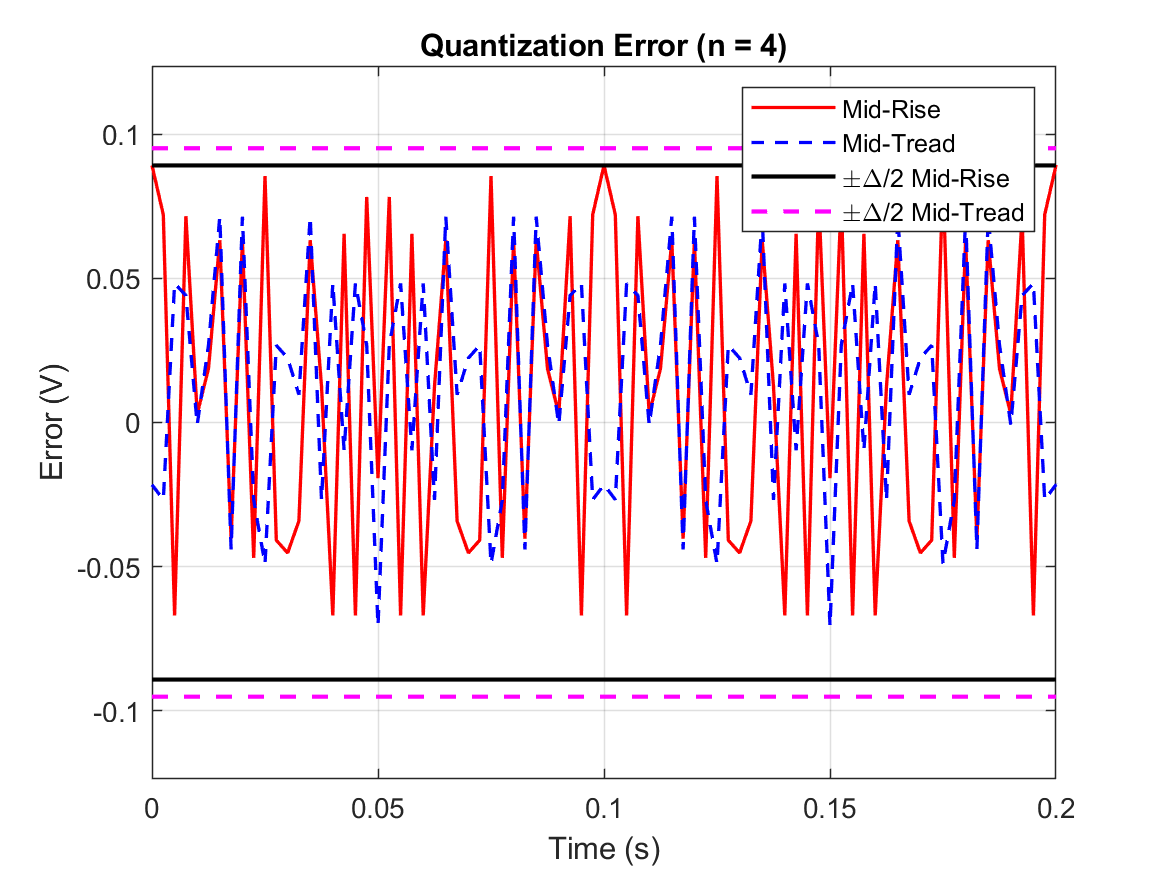
\includegraphics[width=\textwidth]{Octave Scripts/digA_item4_5_figures/Quantization_Error_n_4.png}
        \caption{$n = 4$ bits ($L = 16$)}
    \end{subfigure}\\[0.6em]
    \begin{subfigure}[b]{0.48\textwidth}
        \centering
        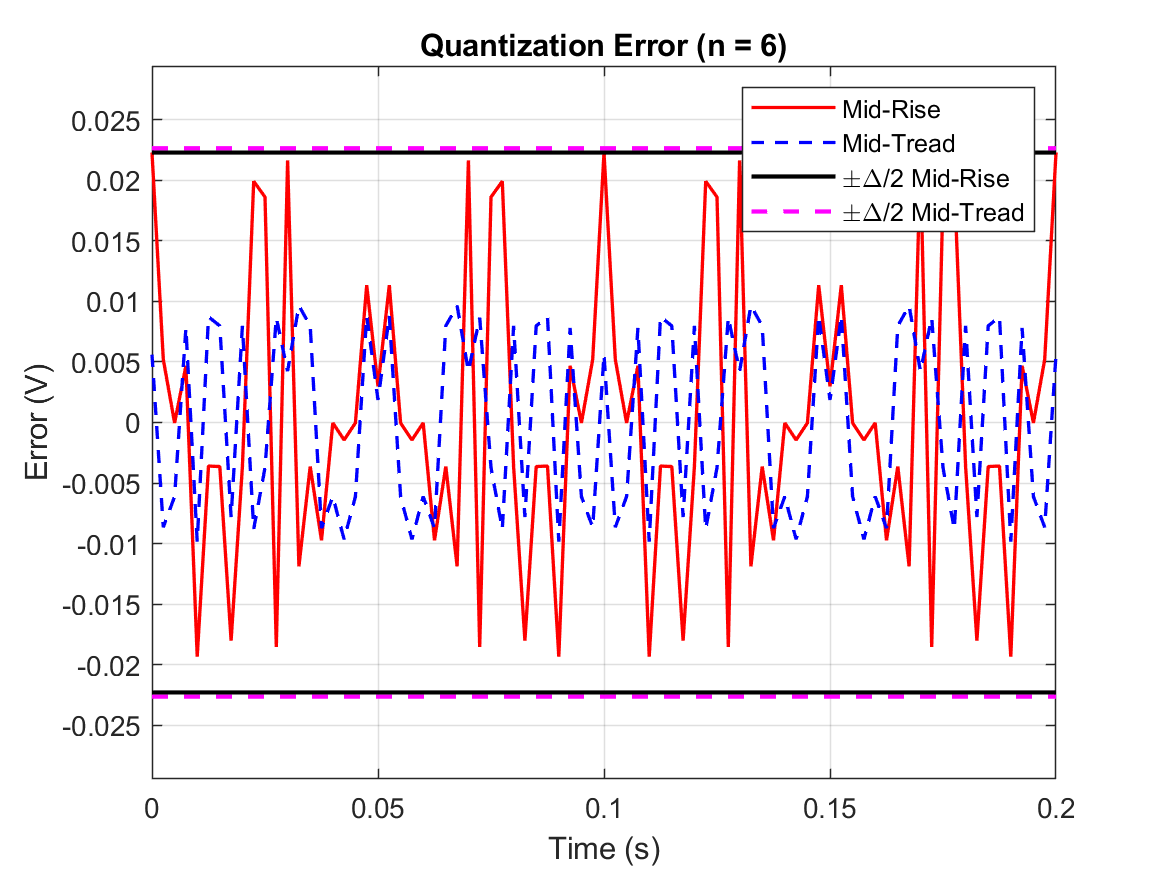
\includegraphics[width=\textwidth]{Octave Scripts/digA_item4_5_figures/Quantization_Error_n_6.png}
        \caption{$n = 6$ bits ($L = 64$)}
    \end{subfigure}\hfill
    \begin{subfigure}[b]{0.48\textwidth}
        \centering
        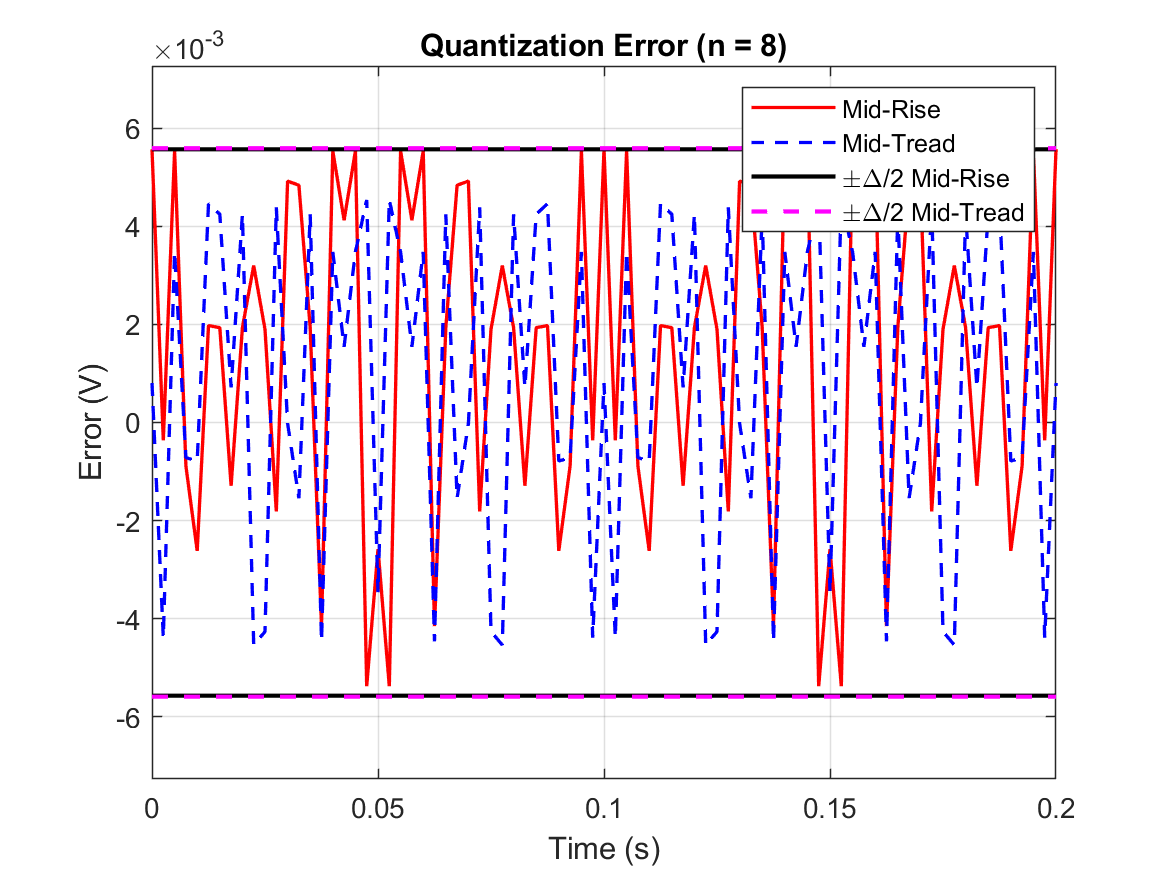
\includegraphics[width=\textwidth]{Octave Scripts/digA_item4_5_figures/Quantization_Error_n_8.png}
        \caption{$n = 8$ bits ($L = 256$)}
    \end{subfigure}
    \caption{Item 4(a): Quantization error $e(t) = m(t) - m_q(t)$ for Mid-Rise and Mid-Tread quantizers across $n \in \{3, 4, 6, 8\}$ bits, overlaid with each quantizer's $\pm\Delta/2$ bounds.}
    \label{fig:digA_item4_errors}
\end{figure}

\paragraph{Item 4(b): Verification that $|e(t)| \le \Delta / 2$.}
Because every input sample in $[V_{\min}, V_{\max}]$ is rounded to its closest reconstruction level (spaced by $\Delta$), the granular error magnitude cannot exceed $\Delta / 2$. Table~\ref{tab:digA_item4_bounds} confirms from simulation that $\max|e(t)| \le \Delta/2$ holds in every case (for Mid-Rise, $\max|e|$ reaches $\Delta_{\text{rise}}/2$ at $t = 0$, where $m(0) = V_{\max}$ lies on the upper cell boundary).

\begin{table}[H]
\centering
\caption{Verification of $|e(t)| \le \Delta/2$ ($R = 2.8529\text{ V}$, $f_s = 400\text{ Hz}$)}
\label{tab:digA_item4_bounds}
\begin{tabular}{c c c c c c c}
\toprule
\textbf{$n$} & \textbf{$L = 2^n$} & \textbf{$\Delta_{\text{rise}}/2$ (V)} & \textbf{$\max|e_{\text{rise}}|$ (V)} & \textbf{$\Delta_{\text{tread}}/2$ (V)} & \textbf{$\max|e_{\text{tread}}|$ (V)} & \textbf{Bound Valid?} \\
\midrule
3 & 8   & 0.17831 & 0.17831 & 0.20378 & 0.19098 & Yes \\
4 & 16  & 0.08915 & 0.08915 & 0.09510 & 0.07138 & Yes \\
6 & 64  & 0.02229 & 0.02229 & 0.02264 & 0.00984 & Yes \\
8 & 256 & 0.00557 & 0.00557 & 0.00559 & 0.00454 & Yes \\
\bottomrule
\end{tabular}
\end{table}

\paragraph{Item 4(c): Simulated vs.\ Theoretical SQNR.}
Modeling the quantization error as uniformly distributed over $[-\Delta/2, +\Delta/2]$ gives noise power $P_q = \Delta^2 / 12$. For Mid-Rise ($\Delta_{\text{rise}} = R/2^n$):
\begin{equation}
\text{SQNR}_{\text{theo, rise}}(\text{dB}) = 10\log_{10}\!\left(\frac{P_{\text{sig}}}{\Delta_{\text{rise}}^2 / 12}\right) = 20\log_{10}(2)\,n + 10\log_{10}\!\left(\frac{12 P_{\text{sig}}}{R^2}\right) = 6.02\,n - 0.36\text{ dB}
\end{equation}
while for Mid-Tread, $\Delta_{\text{tread}} = R/(2^n - 1)$ gives $\text{SQNR}_{\text{theo, tread}}(\text{dB}) = 10\log_{10}(12 P_{\text{sig}} / \Delta_{\text{tread}}^2)$. Note that the constant is $-0.36\text{ dB}$ rather than $+1.76\text{ dB}$ because $+1.76\text{ dB}$ applies only to a single full-scale sinusoid, whereas our asymmetric two-tone message has a higher peak-to-average ratio.

\begin{table}[H]
\centering
\caption{Simulated vs.\ Theoretical SQNR for $n = 3, 4, 6,$ and $8$ bits ($f_s = 400\text{ Hz}$)}
\label{tab:digA_item4_sqnr}
\begin{tabular}{c c c c c}
\toprule
\textbf{$n$ (bits)} & \textbf{Mid-Rise Sim (dB)} & \textbf{Mid-Rise Theory (dB)} & \textbf{Mid-Tread Sim (dB)} & \textbf{Mid-Tread Theory (dB)} \\
\midrule
3 & 16.04 & 17.71 & 16.15 & 16.55 \\
4 & 22.72 & 23.73 & 25.37 & 23.17 \\
6 & 36.24 & 35.77 & 40.13 & 35.63 \\
8 & 46.76 & 47.81 & 47.15 & 47.78 \\
\bottomrule
\end{tabular}
\end{table}

\begin{figure}[H]
    \centering
    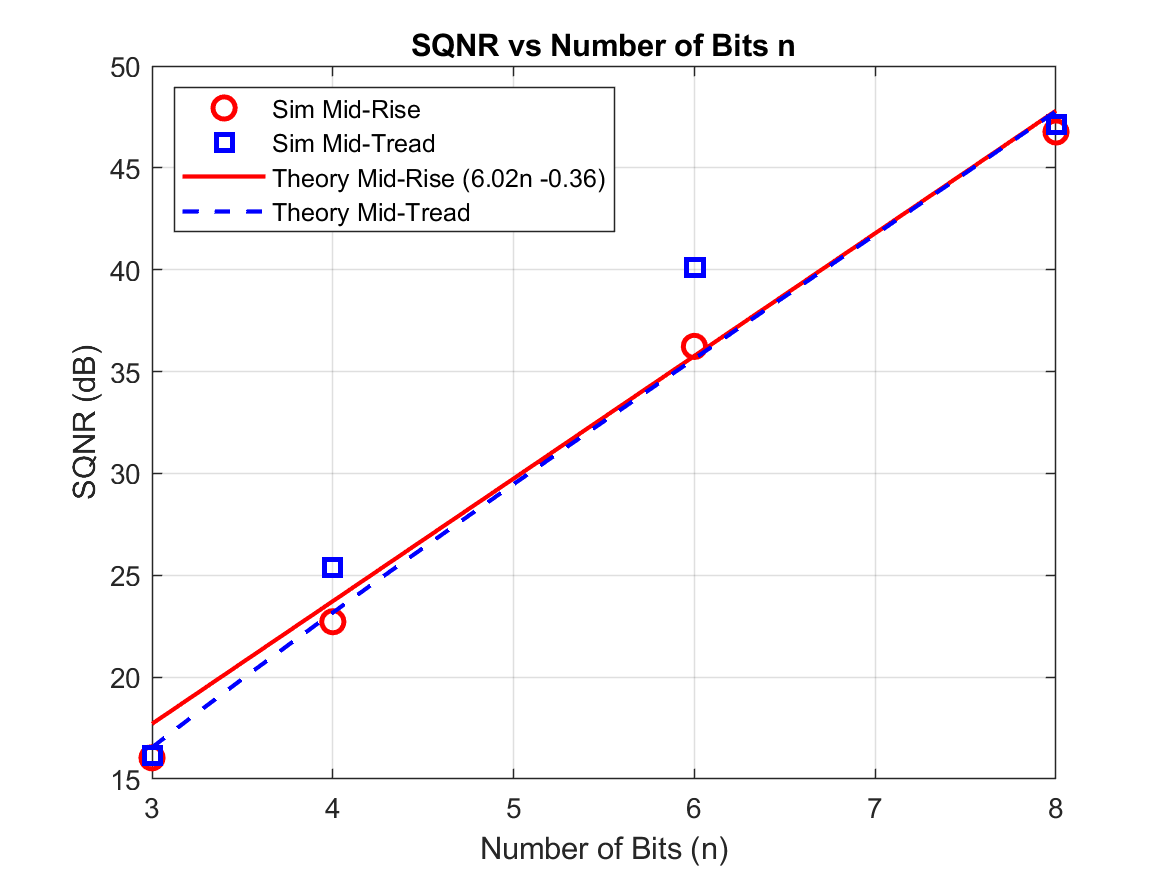
\includegraphics[width=0.72\textwidth]{Octave Scripts/digA_item4_5_figures/SQNR_vs_Number_of_Bits_n.png}
    \caption{Item 4(c): Simulated and theoretical SQNR versus number of bits $n$ for Mid-Rise and Mid-Tread quantizers.}
    \label{fig:digA_item4_sqnr}
\end{figure}

\noindent\textbf{Do they agree? If not, why?} Both simulated curves follow the theoretical $\approx 6.02\text{ dB/bit}$ slope closely. Minor deviations ($0.4\text{--}4.5\text{ dB}$) arise because: (1) at low bit depths ($n = 3, 4$), $\Delta$ is coarse so $e(t)$ is deterministic and correlated with $m(t)$ rather than uniform white noise; and (2) at $f_s = 400\text{ Hz}$ with $f_0 = 10\text{ Hz}$, one period contains only $f_s / f_0 = 40$ unique sample values (repeated 10 times in $1\text{ s}$), including $m(0) = V_{\max}$ hitting the cell boundary with worst-case error $\Delta/2$ every cycle in Mid-Rise.

\paragraph{Item 4(d): Minimum Bits for $\text{SQNR} \ge 40\text{ dB}$.}
From the theoretical relation, $6.0206\,n - 0.355 \ge 40 \implies n \ge 6.70 \implies n_{\min} = \lceil 6.70 \rceil = 7\text{ bits}$. Verifying by simulation at $f_s = 400\text{ Hz}$:
\begin{itemize}
    \item \textbf{$n = 7$ bits ($L = 128$):} \textbf{Mid-Tread achieves $41.77\text{ dB} \ge 40\text{ dB}$} (passes), whereas Mid-Rise gives $39.91\text{ dB}$ ($0.09\text{ dB}$ short of $40\text{ dB}$ due to the 40-sample grid alignment; on a dense waveform it achieves $41.73\text{ dB}$).
    \item \textbf{$n = 8$ bits ($L = 256$):} Mid-Rise achieves $46.76\text{ dB}$ and Mid-Tread achieves $47.15\text{ dB}$ (both strictly exceed $40\text{ dB}$).
\end{itemize}
Hence, \textbf{$n = 7$ bits with Mid-Tread quantization} satisfies $\text{SQNR} \ge 40\text{ dB}$ at the lowest bit rate and bandwidth, and is selected for Item~5.

\subsubsection{PCM Encoding, Decoding, and Bandwidth Analysis (Item 5)}

\paragraph{PCM Encoder and Decoder Verification.}
Using the $n = 7$-bit Mid-Tread quantizer ($L = 128$, $k_{\min} = -60$), each quantized sample is mapped to an unsigned integer index $\text{idx} = k_{\text{tread}} - k_{\min} \in \{0, 1, \dots, 127\}$ and encoded (MSB first) via positional base-2 math:
\begin{equation}
b_j = \left\lfloor \frac{\text{idx}}{2^j} \right\rfloor \bmod 2, \qquad j = 6, 5, \dots, 0
\end{equation}
Serializing all $N_s = 400$ codewords yields a $1 \times 2800$ binary stream (Figure~\ref{fig:digA_item5_plots}a shows the first 3 samples $= 21$ bits: $\text{idx} = 127 \to [1111111]$, $\text{idx} = 118 \to [1110110]$, $\text{idx} = 96 \to [1100000]$). At the receiver, framing the serial stream back into 7-bit words, computing $\widehat{\text{idx}} = \sum_{j=0}^{6} b_j 2^j$, and reconstructing $\hat{m}_q = (\widehat{\text{idx}} + k_{\min})\Delta_{\text{tread}}$ produces \textbf{0 index mismatches} out of 400 samples and $\max|\hat{m}_q - m_q| = 0\text{ V}$ (Figure~\ref{fig:digA_item5_plots}b).

\begin{figure}[H]
    \centering
    \begin{subfigure}[b]{0.48\textwidth}
        \centering
        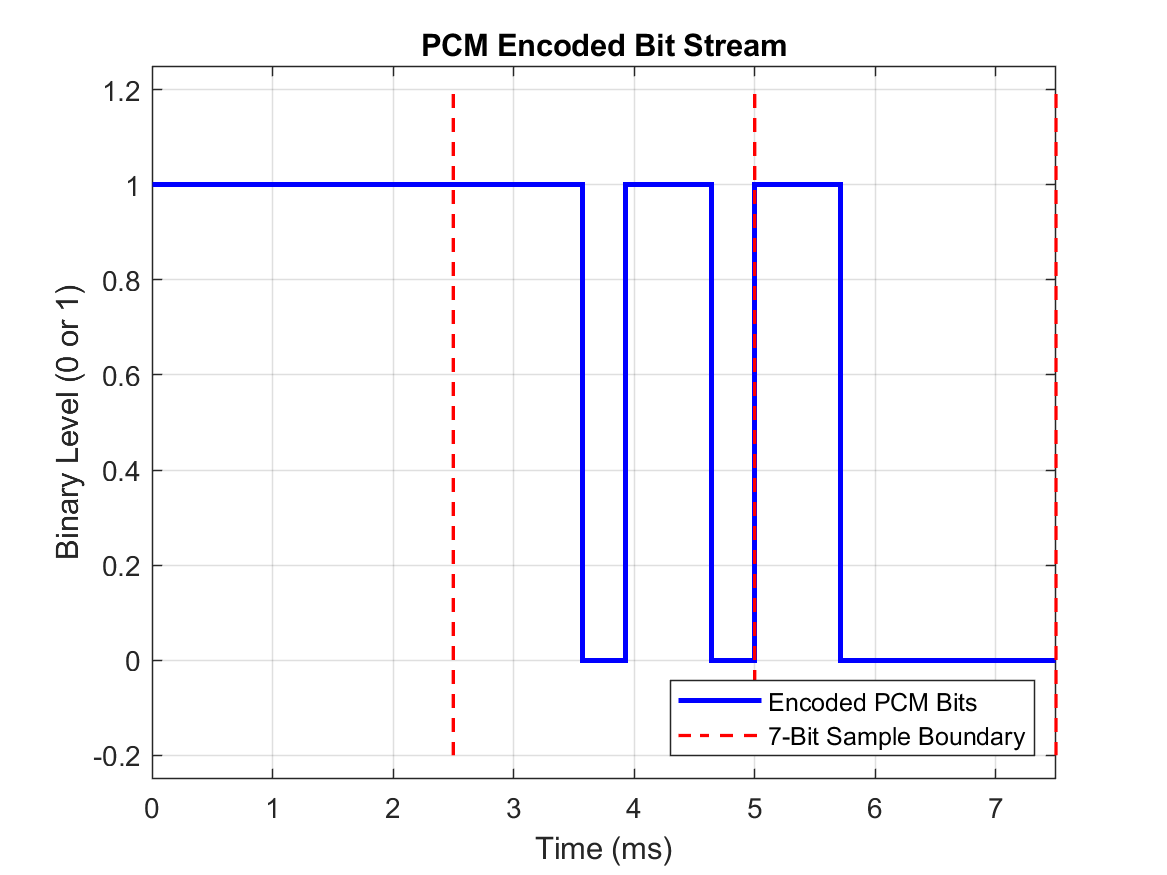
\includegraphics[width=\textwidth]{Octave Scripts/digA_item4_5_figures/PCM_Encoded_Bit_Stream.png}
        \caption{Encoded PCM bit stream (first 3 samples $= 21$ bits)}
    \end{subfigure}\hfill
    \begin{subfigure}[b]{0.48\textwidth}
        \centering
        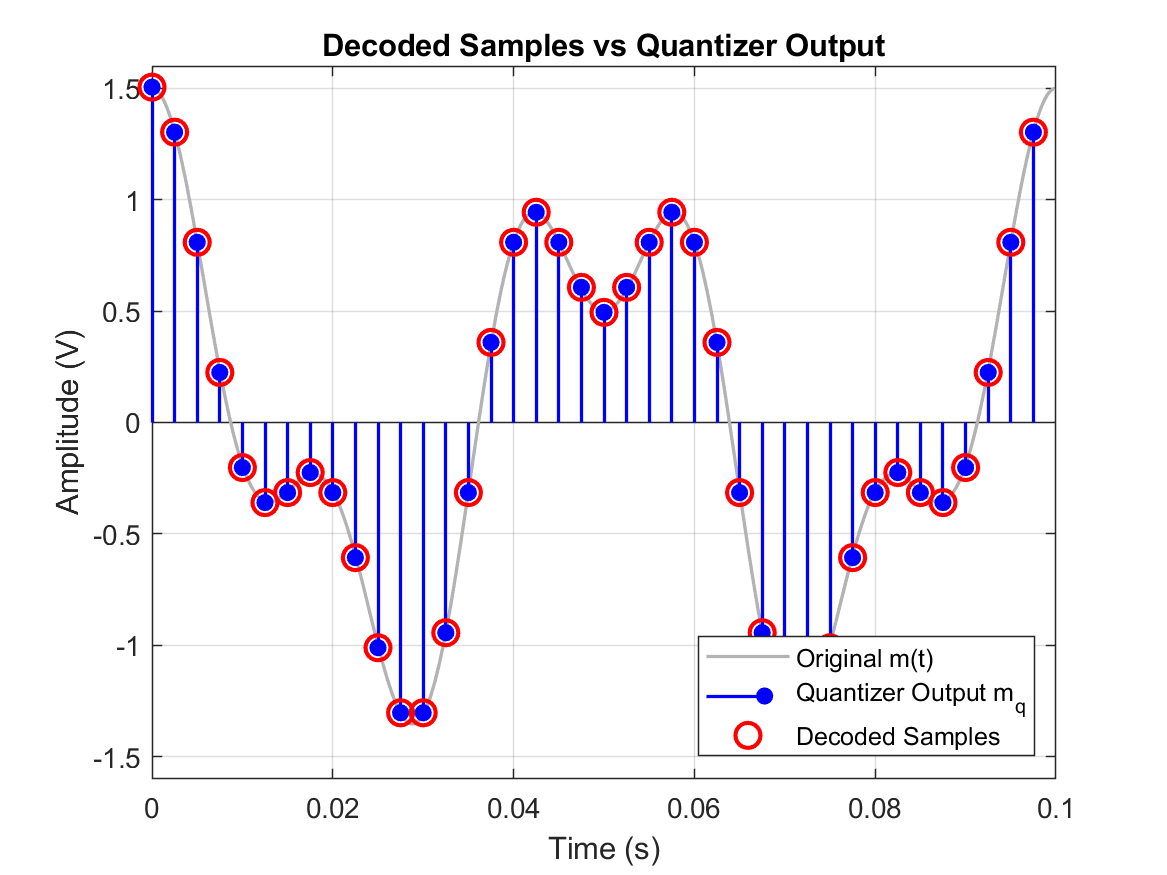
\includegraphics[width=\textwidth]{Octave Scripts/digA_item4_5_figures/Decoded_Samples_vs_Quantizer_Output.png}
        \caption{Decoded samples $\hat{m}_q$ overlaid on quantizer output $m_q$}
    \end{subfigure}
    \caption{Item 5: (a) Serialized 7-bit PCM binary stream ($T_b = 0.3571\text{ ms}$) and (b) exact agreement between decoded samples and quantizer output over one period ($0.1\text{ s}$).}
    \label{fig:digA_item5_plots}
\end{figure}

\paragraph{Bit Rate, Minimum Transmission Bandwidth, and the Price of Digital Transmission.}
For $f_s = 400\text{ Hz}$ ($4\times$ Nyquist) and $n = 7\text{ bits/sample}$:
\begin{equation}
R_b = n \cdot f_s = 7 \times 400 = 2800\text{ bits/s} \quad (T_b = 0.3571\text{ ms}), \qquad B_{\text{PCM, min}} = \frac{R_b}{2} = 1400\text{ Hz}
\end{equation}
Compared to the original analog message bandwidth $W = 50\text{ Hz}$, the minimum Nyquist zero-ISI bandwidth of the PCM signal is $\mathbf{1400 / 50 = 28\times W}$ (and even at exact Nyquist sampling $f_s = 2W = 100\text{ Hz}$, $R_b = 700\text{ bits/s}$ and $B_{\text{PCM, min}} = nW = 350\text{ Hz} = \mathbf{7\times W}$).

\noindent\textbf{The Price of Digital Transmission:} Digital PCM trades \textbf{bandwidth expansion} (requiring at least $n\times W$, and $28\times W$ here, plus A/D and synchronization hardware) in exchange for \textbf{regenerative noise immunity} over long links (repeaters eliminate cumulative noise), \textbf{exponential SQNR improvement with bandwidth} ($+6.02\text{ dB}$ per bit), and straightforward TDM multiplexing, error-control coding, and encryption.

\begin{table}[H]
\centering
\caption{Summary of Numerical Results for Digital Part A, Items 4 and 5}
\label{tab:digA_item4_5_summary}
\begin{tabular}{l c}
\toprule
\textbf{Parameter / Metric} & \textbf{Value} \\
\midrule
Message Extreme Values ($V_{\max}$ / $V_{\min}$) & $+1.5000\text{ V}$ / $-1.3529\text{ V}$ \\
Asymmetric Dynamic Range ($R = V_{\max} - V_{\min}$) & $2.8529\text{ V}$ \\
Average Message Power ($P_{\text{sig}}$) & $0.6250\text{ W}$ \\
Minimum Bits for $\text{SQNR} \ge 40\text{ dB}$ ($n$) & $7\text{ bits}$ (Mid-Tread Sim: $41.77\text{ dB}$) \\
PCM Sampling Rate ($f_s$) / Bit Rate ($R_b = n f_s$) & $400\text{ Hz}$ / $2800\text{ bits/s}$ \\
Minimum PCM Bandwidth ($B_{\text{PCM, min}} = R_b/2$) & $1400\text{ Hz}$ ($= 28\times W$, vs.\ $W = 50\text{ Hz}$) \\
Min.\ PCM Bandwidth at Exact Nyquist ($f_s = 100\text{ Hz}$) & $350\text{ Hz}$ ($= 7\times W$, $R_b = 700\text{ bits/s}$) \\
Decoder Sample / Bit Errors (Noiseless Link) & $0 / 400$ samples ($\max|\hat{m}_q - m_q| = 0\text{ V}$) \\
\bottomrule
\end{tabular}
\end{table}

\noindent\textbf{Octave Implementation (Items 4 and 5).}\par\smallskip
\begin{lstlisting}[basicstyle=\ttfamily\scriptsize, breaklines=true, breakatwhitespace=true, frame=single, xleftmargin=6pt, xrightmargin=6pt, framexleftmargin=6pt, framexrightmargin=6pt, aboveskip=4pt, belowskip=6pt]
% ECE 351s - Digital Communication Part A: Items 4 & 5 (Core Logic)
clear; close all; clc;

%% Message Signal (fs = 400 Hz = 4x Nyquist) & True Asymmetric Range
fs = 400; Ts = 1 / fs;
t  = 0 : Ts : 1 - Ts;                         % 1 s = 400 samples
m  = cos(2*pi*20*t) + 0.5*cos(2*pi*50*t);

td   = 0 : 1/8000 : 0.1 - 1/8000;             % Fine grid for true Vmax/Vmin
md   = cos(2*pi*20*td) + 0.5*cos(2*pi*50*td);
Vmax = max(md); Vmin = min(md); R = Vmax - Vmin;
Psig = mean(m.^2);

%% Item 4(a) & 4(b): Mid-Tread & Mid-Rise Quantizers and Error Bound Check
n_values   = [3, 4, 6, 8];
SQNR_rise  = zeros(1, length(n_values));
SQNR_tread = zeros(1, length(n_values));

for i = 1:length(n_values)
    n = n_values(i); L = 2^n;

    % Mid-Tread Quantizer (zero is a reconstruction level)
    Delta_tread = R / (L - 1);
    kmin  = round(Vmin / Delta_tread);
    tread = round(m / Delta_tread);
    tread(tread > kmin + L - 1) = kmin + L - 1;
    tread(tread < kmin)         = kmin;
    mq_tread  = tread * Delta_tread;
    err_tread = m - mq_tread;

    % Mid-Rise Quantizer (zero is a decision threshold)
    Delta_rise = R / L;
    rise = floor((m - Vmin) / Delta_rise);
    rise(rise > L - 1) = L - 1;
    rise(rise < 0)     = 0;
    mq_rise  = Vmin + (rise + 0.5) * Delta_rise;
    err_rise = m - mq_rise;

    % Item 4(b): Verify |error| <= Delta/2
    max_err_rise  = max(abs(err_rise));
    max_err_tread = max(abs(err_tread));
    valid_rise    = max_err_rise  <= Delta_rise/2 * (1 + 1e-9);
    valid_tread   = max_err_tread <= Delta_tread/2 * (1 + 1e-9);

    SQNR_rise(i)  = 10 * log10(Psig / mean(err_rise.^2));
    SQNR_tread(i) = 10 * log10(Psig / mean(err_tread.^2));
end

%% Item 4(c): Theoretical SQNR Expressions
n_plot   = 3 : 0.1 : 8;
const_dB = 10 * log10(12 * Psig / R^2);
theo_SQNR_rise  = 20*log10(2) .* n_plot + const_dB;
theo_SQNR_tread = 10 * log10(Psig ./ ((R ./ (2.^n_plot - 1)).^2 / 12));

%% Item 4(d): Minimum Bits Required for SQNR >= 40 dB & Simulation Check
n_target = ceil((40 - const_dB) / (20 * log10(2)));   % ceil(6.70) = 7 bits
for n_test = [n_target, n_target + 1]
    L_t = 2^n_test;
    Dr  = R / L_t;
    r_idx  = min(max(floor((m - Vmin) / Dr), 0), L_t - 1);
    mq_r   = Vmin + (r_idx + 0.5) * Dr;
    sqnr_r = 10 * log10(Psig / mean((m - mq_r).^2));

    Dt    = R / (L_t - 1); km = round(Vmin / Dt);
    t_idx = min(max(round(m / Dt), km), km + L_t - 1);
    mq_t  = t_idx * Dt;
    sqnr_t = 10 * log10(Psig / mean((m - mq_t).^2));
end

%% Item 5: 7-Bit Mid-Tread PCM Encoder, Decoder & Bandwidth Analysis
Ns = length(m); n_pcm = n_target; L_pcm = 2^n_pcm;
Delta_pcm = R / (L_pcm - 1);
kmin_pcm  = round(Vmin / Delta_pcm);
tread_pcm = min(max(round(m / Delta_pcm), kmin_pcm), kmin_pcm + L_pcm - 1);
mq_pcm    = tread_pcm * Delta_pcm;
idx_pcm   = tread_pcm - kmin_pcm;                     % {0, 1, ..., 127}

% Natural Binary PCM Encoder (MSB first)
codewords = zeros(Ns, n_pcm);
for b = 1:n_pcm
    codewords(:, b) = mod(floor(idx_pcm / 2^(n_pcm - b)), 2);
end
pcm_bits = reshape(codewords.', 1, []);               % 1 x 2800 serial stream

% PCM Decoder & Verification
codewords_rx = reshape(pcm_bits, n_pcm, []).';
idx_decoded  = zeros(1, Ns);
for b = 1:n_pcm
    idx_decoded = idx_decoded + codewords_rx(:, b).' * 2^(n_pcm - b);
end
mq_decoded     = (idx_decoded + kmin_pcm) * Delta_pcm;
num_idx_errors = sum(idx_decoded ~= idx_pcm);         % = 0
max_amp_diff   = max(abs(mq_decoded - mq_pcm));       % = 0

% Bit Rate and Minimum Transmission Bandwidth
W  = 50; Rb = n_pcm * fs; BW_pcm_min = Rb / 2; BW_ratio = BW_pcm_min / W;
fs_nyq = 2 * W; Rb_nyq = n_pcm * fs_nyq; BW_nyq_min = Rb_nyq / 2;
\end{lstlisting}

\subsection{Line Coding and Digital Modulation}
\subsubsection{Line Coding}
\noindent\textbf{a.} To be able to compare AMI with polar NRZ, we first need to simulate them using Octave. In our simulation we assumed that the pulse width $T_b=1$ second (to get a normalized frequency spectrum) and that there are $\frac{1}{dt}$ samples per pulse.
\begin{lstlisting}
AMI = [];
high = 1;

P_NRZ = [];
for (d = bit_stream)
  AMI = [AMI,  d*high*ones(1, 1/(2*dt)), zeros(1, 1/(2*dt))];
  high *= (-1)^d;

  P_NRZ = [P_NRZ, (2*d-1)*ones(1, 1/dt)];
endfor
\end{lstlisting}

\noindent\textbf{b.} The waveforms of 64 randomly generated bits are shown in the next figure.

\begin{figure}[H]
  \centering
  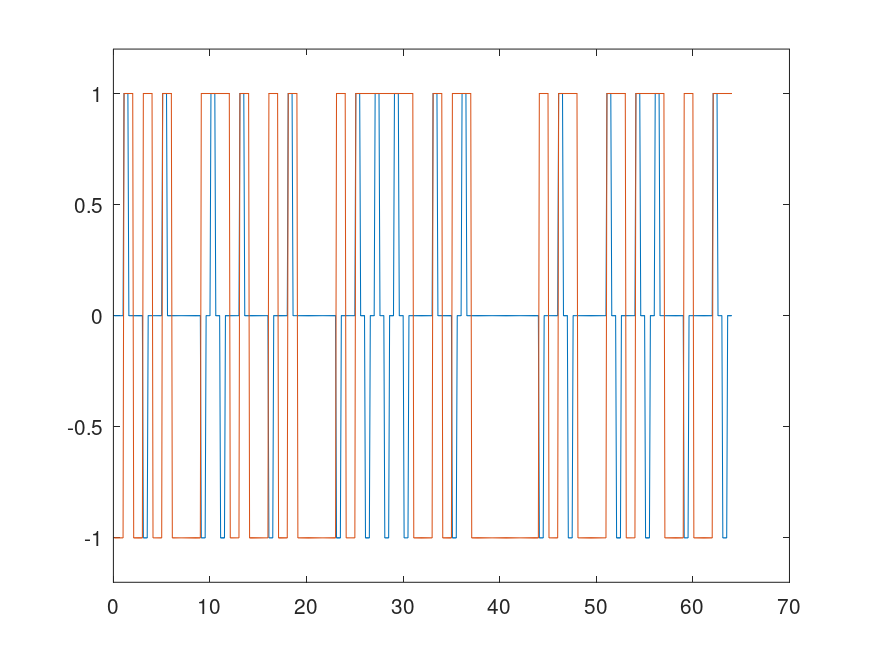
\includegraphics[width=0.9\textwidth]{Octave Scripts/digB_1_figures/time_domain_waveform.png}
  \caption{Time-domain waveforms of AMI and Polar NRZ for 64 random bits.}
\end{figure}

\noindent To get an accurate power spectral density (\textit{PSD}), we randomly generated a 16384-bit stream which was used to compute the spectra. After calculating the spectra we obtained the PSDs shown in the next figure.

\begin{figure}[H]
  \centering
  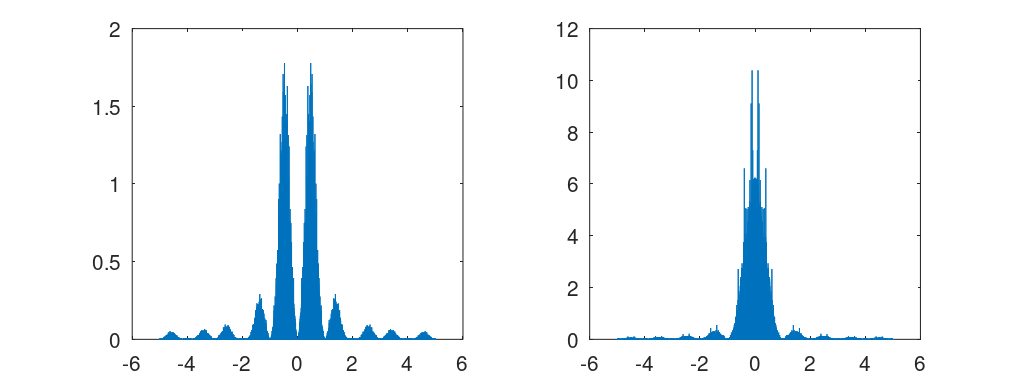
\includegraphics[width=\textwidth]{Octave Scripts/digB_1_figures/Power_16384bits.png}
  \caption{Power spectral density (PSD) of AMI and Polar NRZ computed over 16384 bits.}
\end{figure}

\noindent\textbf{c.} The first null for both line codes occurs at unity for $T_b = 1$; generally, the first null is at $\frac{1}{T_b}$ for both. Neither one contains a DC component, but polar NRZ has significant power spectrum at low frequencies, which can cause information loss in transformer-coupled circuits since they filter out low frequencies. On the other hand, AMI has low power spectrum at low frequencies, so it provides more reliable transmission over AC-coupled channels.

\medskip
\noindent\textbf{d.} We can see in the next figure that for the pattern \texttt{10101010} the clock can be recovered from either line code. However, for the pattern \texttt{11111111}, we can only recover the clock from AMI since it returns to zero and has alternating polarity making each individual pulse distinguishable, while polar NRZ produces a constant HIGH signal. For the pattern \texttt{00000000}, the clock can \textit{not} be recovered from either of them since both produce a constant signal. Neither of the line codes is fully transparent, but AMI is better in this regard.

\begin{figure}[H]
  \centering
  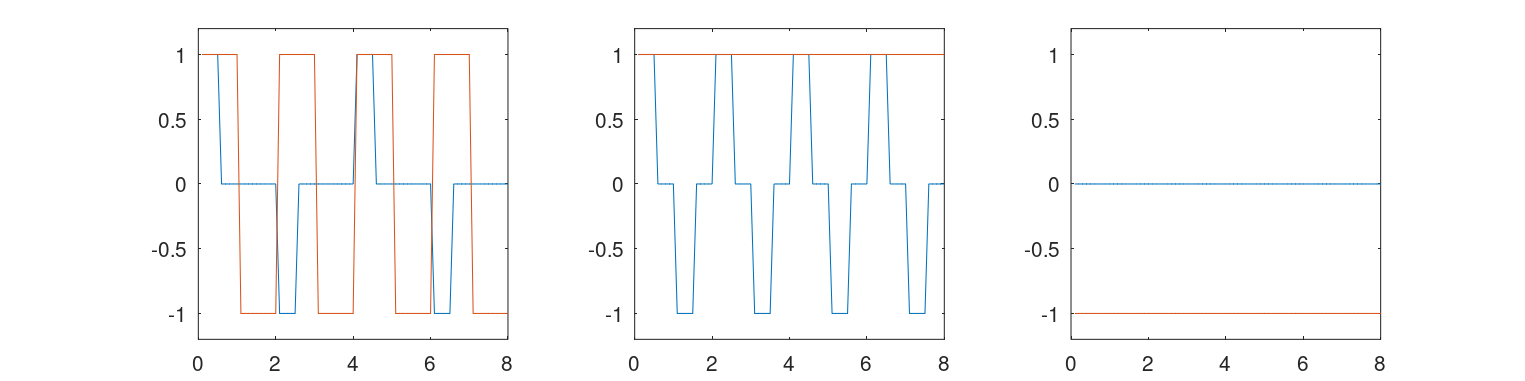
\includegraphics[width=\textwidth]{Octave Scripts/digB_1_figures/CLK_Recovery_Patterns.png}
  \caption{Clock recovery comparison of AMI and Polar NRZ for the bit patterns \texttt{10101010}, \texttt{11111111}, and \texttt{00000000}.}
\end{figure}

\noindent\textbf{e.} Both line codes have their respective advantages: AMI is better for error detection and transmission over AC-coupled channels, while polar NRZ has better noise margins due to the larger difference between its levels. For a real link I would choose AMI since it is better for transmission, has error detection capability, and is more transparent.


% =====================================================================
% Digital Part B, Item 2 -- Digital Modulation (BPSK)
% Paste this block into Report.tex right after the "Line Coding"
% subsubsection (before \end{document}).
% Needs no new packages. Figures are read from
%   Octave Scripts/digB_2_figures/   (same relative style as the other items)
% =====================================================================
\subsubsection{Digital Modulation (BPSK)}
Our group selected \textbf{binary phase-shift keying (BPSK)} for the digital modulation item. The line code compared in Item~1 is AMI against polar NRZ, so AMI is the line code used in part~(e). We kept the normalized units of Item~1: bit duration $T_b = 1$ second, so the bit rate is $R_b = 1$ bit/s and every frequency below can also be read in units of $R_b$. The carrier is $f_c = 10$ Hz, which is higher than the bit rate as required (ten full carrier cycles per bit), with amplitude $A = 1$ V. The bit stream has 64 bits and is generated randomly by the program. The simulation grid is 1000 Hz (1000 samples per bit). The modulator, mixer, low-pass filter (LPF), bit decision and power spectral density (PSD) estimator are all written by hand, with no communication-toolbox functions.

\medskip
\noindent\textbf{a.} \textit{Transmitter and coherent receiver.} In BPSK the carrier phase is $0$ for a bit 1 and $\pi$ for a bit 0, which is the product of the polar NRZ waveform $b(t) = \pm 1$ of Item~1 and the carrier:
\begin{equation}
s(t) = A\, b(t) \cos(2\pi f_c t)
\end{equation}
The coherent receiver multiplies the received signal by a local oscillator (LO) $2\cos(2\pi f_c t + \phi)$, where $\phi$ is the LO phase error:
\begin{equation}
v(t) = s(t)\cdot 2\cos(2\pi f_c t + \phi) = A\, b(t)\left[\cos\phi + \cos(4\pi f_c t + \phi)\right]
\end{equation}
An ideal LPF (a brick-wall mask applied in the frequency domain, cut-off $4R_b = 4$ Hz) removes the term at $2f_c = 20$ Hz and leaves $y(t) = A\, b(t) \cos\phi$. The decision device samples $y(t)$ in the middle of every bit and decides bit 1 if the sample is positive and bit 0 otherwise.
\begin{lstlisting}
s = A*b.*cos(2*pi*fc*t);                          % BPSK transmitter
for i = 1:numel(phis)
  v = s .* (2*cos(2*pi*fc*t + phis(i)*pi/180));   % coherent detector: mixer
  y(i,:) = applyH(v, Hlp);                        % ideal LPF in the frequency domain
  rxBits(i,:) = double(y(i,mid) > 0);             % mid-bit sample, threshold = 0
  nErr(i) = sum(rxBits(i,:) ~= bits);
end
\end{lstlisting}

\medskip
\noindent\textbf{b.} \textit{Waveforms and spectra.} The next figure shows the transmitter output for the first 8 bits. The carrier phase flips by $180^\circ$ exactly where the data changes between 1 and 0.

\begin{figure}[H]
  \centering
  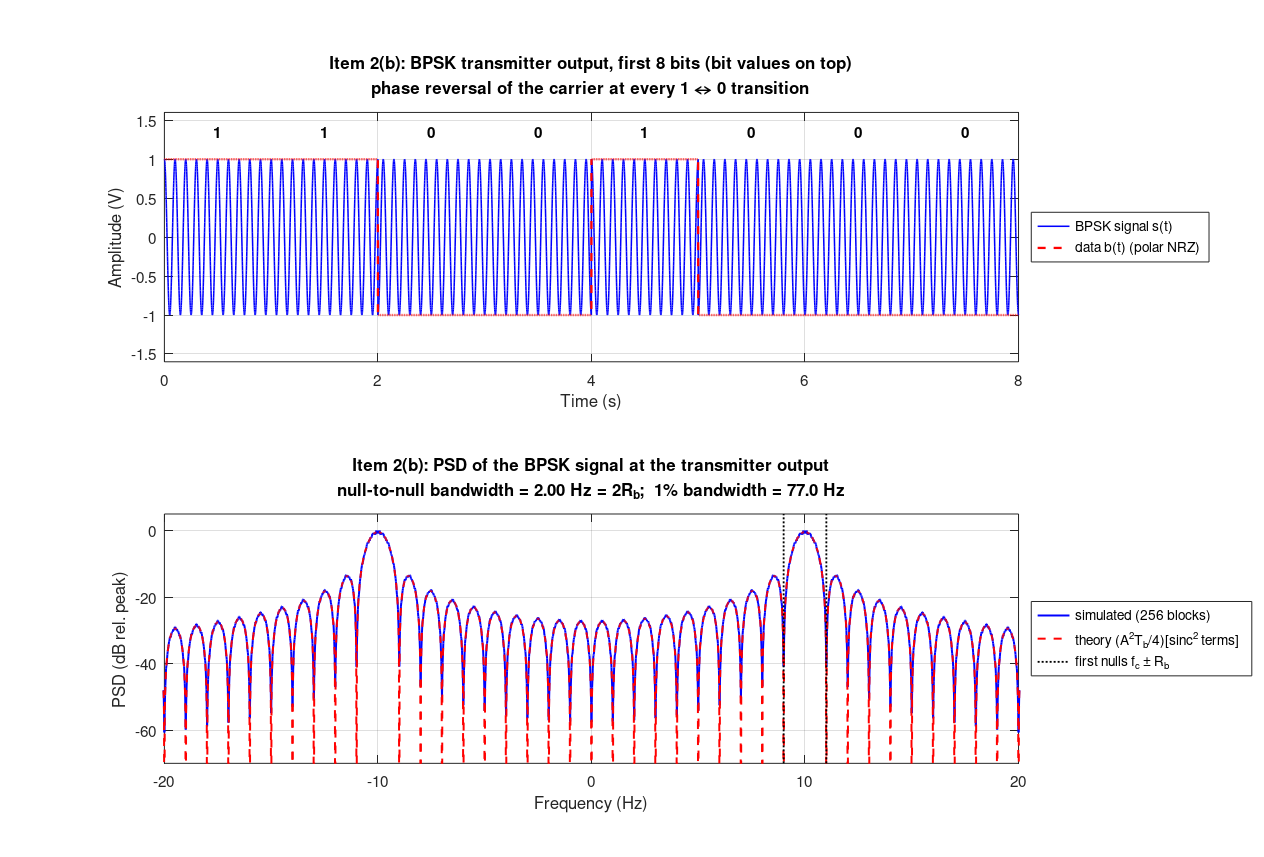
\includegraphics[width=0.95\textwidth]{Octave Scripts/digB_2_figures/01_item2b_tx.png}
  \caption{Item 2(b): BPSK transmitter output $s(t)$ overlaid on the data $b(t)$ for the first 8 bits (top), and PSD of the transmitted signal, simulation overlaid on theory (bottom).}
\end{figure}

\noindent The PSD was obtained by averaging the periodograms of 256 random blocks of 64 bits, each multiplied by a Hann window. Every block uses a random carrier phase. Because $f_c = 10R_b$ is an exact multiple of the bit rate, a carrier locked to the bit clock would make the two spectral images add coherently in the tails and the estimate would sit about 30\% above the textbook formula. A random phase models a link whose carrier has no fixed relation to the bit timing, which is what the standard result assumes. The simulated PSD then agrees with the theory:
\begin{equation}
S_s(f) = \frac{A^2 T_b}{4}\left[\operatorname{sinc}^2\!\big((f - f_c)T_b\big) + \operatorname{sinc}^2\!\big((f + f_c)T_b\big)\right]
\end{equation}
It is the sinc$^2$ spectrum of polar NRZ translated to $\pm f_c$. The first nulls are at $f_c \pm R_b$ (measured at $f_c + 1.000$ Hz), so the \textbf{null-to-null transmission bandwidth is $2R_b = 2$ Hz}, which is the bandwidth required in practice. With the project's 1\% criterion the bandwidth is much larger, $77.0$ Hz from the simulation ($75.1$ Hz from the theory curve), because the sinc tails of rectangular pulses decay slowly: the amplitude spectrum only drops below 1\% of its maximum at about $32R_b$ from the carrier, and the tail of the opposite image adds a little to this.

\noindent The next figure shows the receiver output. The detector output $y(t)$ follows the data apart from the ripple caused by the LPF cut-off. The sampled values are the correct bits, and the PSD at the receiver output is the PSD of the baseband data, which is the PSD of the transmitted $b(t)$ cut at 4 Hz. Its main lobe is $R_b = 1$ Hz wide, half of the passband bandwidth, since the modulation doubled it.

\begin{figure}[H]
  \centering
  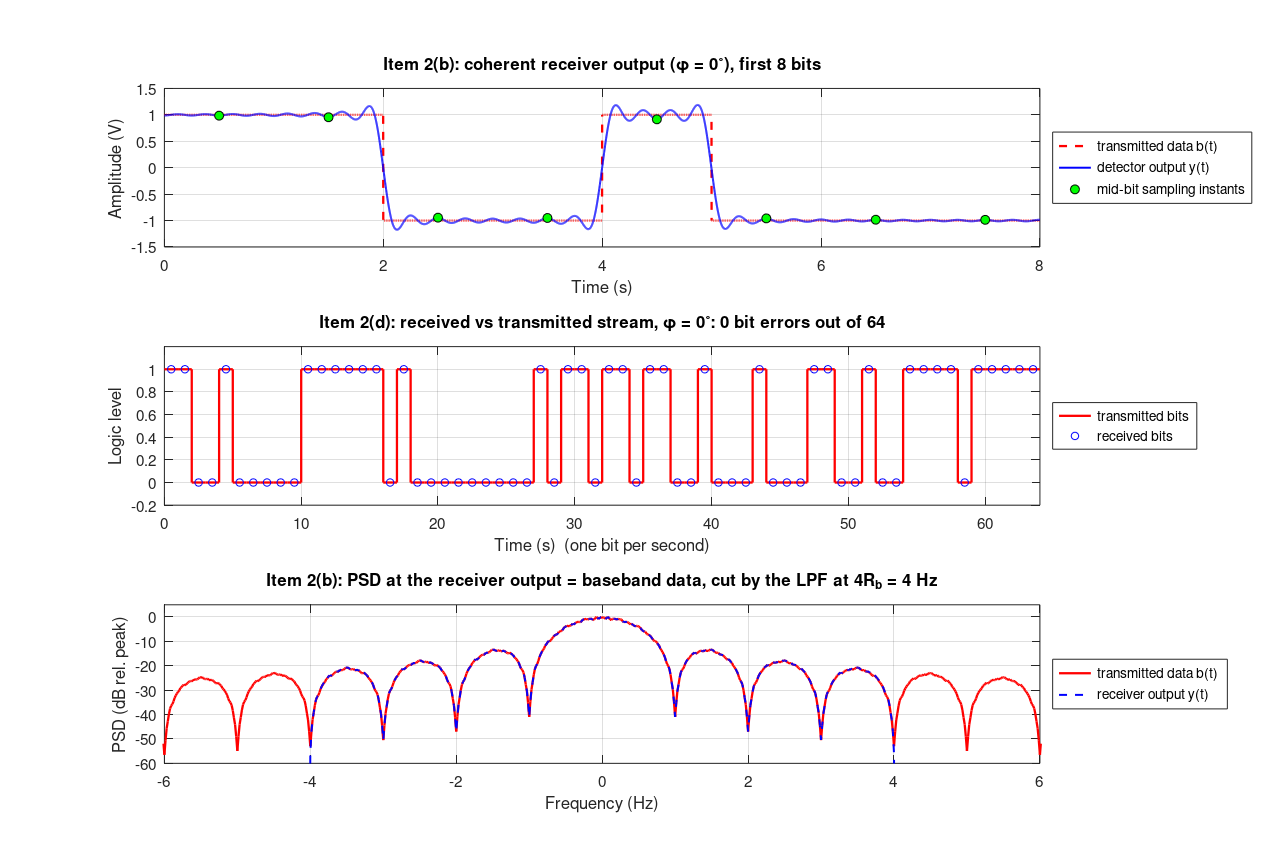
\includegraphics[width=0.95\textwidth]{Octave Scripts/digB_2_figures/02_item2b_rx.png}
  \caption{Items 2(b) and 2(d): coherent receiver output with the mid-bit sampling instants (top), transmitted bits overlaid on received bits (middle), and PSD at the receiver output overlaid on the PSD of the transmitted data (bottom).}
\end{figure}

\medskip
\noindent\textbf{c.} \textit{LO phase error.} After the LPF, $y(t) = A\, b(t)\cos\phi$, so a phase error does not distort the waveform; it scales the detected amplitude by $\cos\phi$ (the measured values relative to the $\phi = 0^\circ$ case agree with $\cos\phi$ to four decimals):
\begin{itemize}
  \item $\phi = 30^\circ$: amplitude $\cos 30^\circ = 0.866$ of the ideal value. The signal is still positive for every 1 and negative for every 0, so the decisions are still correct, but the noise margin falls by $13.4\%$.
  \item $\phi = 60^\circ$: amplitude $\cos 60^\circ = 0.500$. The decisions are still correct, but the margin is halved.
  \item $\phi = 90^\circ$: amplitude $\cos 90^\circ = 0$ (\textbf{quadrature null}). The LO is in quadrature with the carrier, so the mixer output contains only a term at $2f_c$ and the detector output is zero. The decision is made on a value below $7\times 10^{-5}$ V, which is arbitrary.
\end{itemize}
For $\phi > 90^\circ$, $\cos\phi$ is negative and every bit would be detected inverted.

\begin{figure}[H]
  \centering
  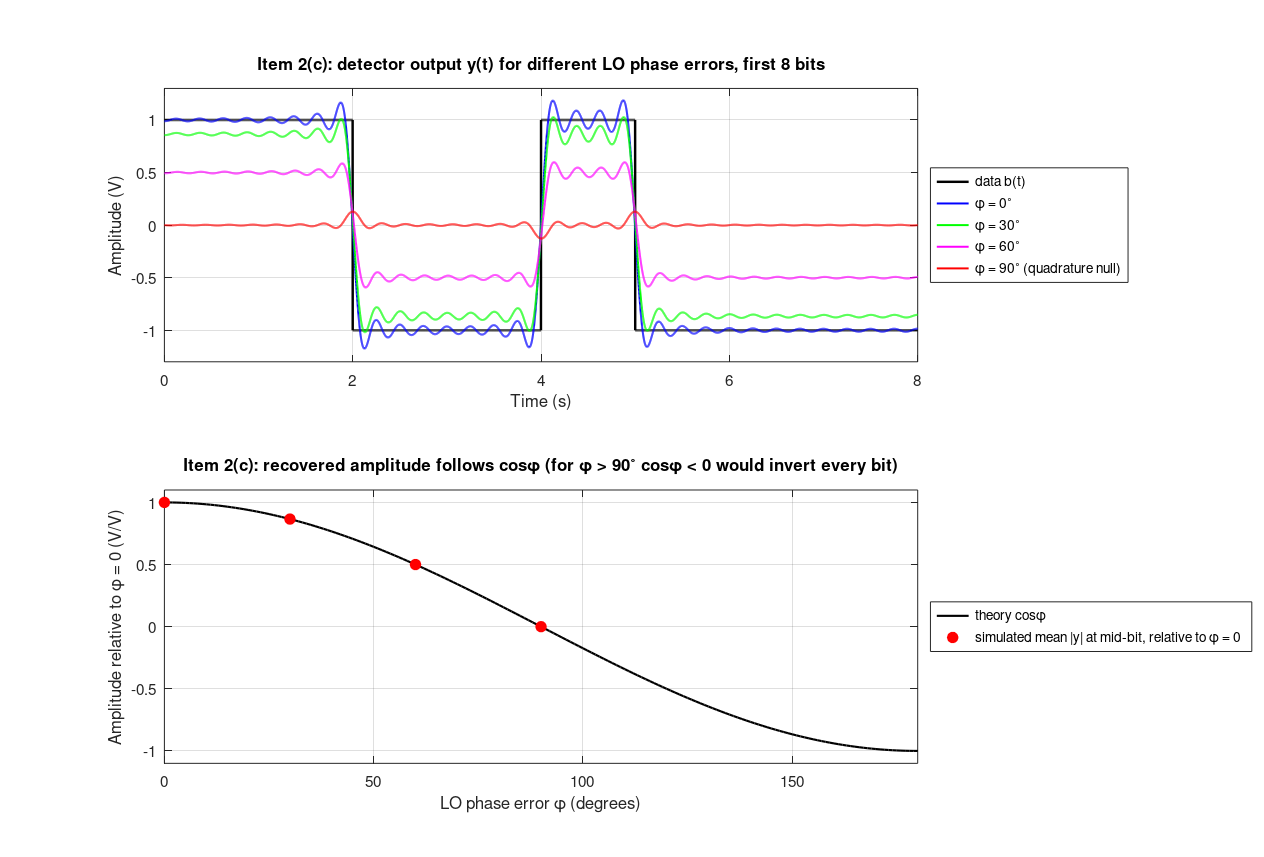
\includegraphics[width=0.95\textwidth]{Octave Scripts/digB_2_figures/03_item2c_phase.png}
  \caption{Item 2(c): detector output for LO phase errors of $0^\circ$, $30^\circ$, $60^\circ$ and $90^\circ$ overlaid on the data (top), and recovered amplitude relative to $\phi = 0^\circ$ overlaid on $\cos\phi$ (bottom).}
\end{figure}

\medskip
\noindent\textbf{d.} \textit{Bit errors.} With the correct oscillator phase the received stream is identical to the transmitted one: \textbf{0 errors out of 64 bits}. With the phase errors of part~(c), the noiseless channel gives $0$ errors for $30^\circ$ and $60^\circ$, because only the amplitude is reduced, and $31$ errors out of 64 for $90^\circ$. The 31 errors at $90^\circ$ are not a meaningful number in themselves: the decisions are made on an essentially zero signal, so each bit is a coin flip and about half of the bits are wrong. The $30^\circ$ and $60^\circ$ cases only show their cost once noise is present. As an extra investigation, we added white Gaussian noise at $E_b/N_0 = 6$ dB and sent 20000 bits through the same receiver (integrate-and-dump detector). The bit error rate then follows $P_e = \tfrac{1}{2}\operatorname{erfc}\!\big(\sqrt{E_b/N_0}\,\cos\phi\big)$, which is equivalent to a loss of $-20\log_{10}\cos\phi$ dB in signal-to-noise ratio ($1.25$ dB at $30^\circ$, $6.02$ dB at $60^\circ$).

\begin{table}[H]
\centering
\caption{Effect of the LO phase error on the BPSK receiver}
\begin{tabular}{c c c c c}
\toprule
\textbf{$\phi$} & \textbf{Amplitude} & \textbf{Errors (no noise)} & \textbf{BER, sim.} & \textbf{BER, theory} \\
\midrule
$0^\circ$  & $1.000$ & 0 / 64  & $2.35\times 10^{-3}$ & $2.39\times 10^{-3}$ \\
$30^\circ$ & $0.866$ & 0 / 64  & $7.30\times 10^{-3}$ & $7.27\times 10^{-3}$ \\
$60^\circ$ & $0.500$ & 0 / 64  & $7.59\times 10^{-2}$ & $7.91\times 10^{-2}$ \\
$90^\circ$ & $0.000$ & 31 / 64 & $0.502$              & $0.500$ \\
\bottomrule
\end{tabular}
\end{table}

\begin{figure}[H]
  \centering
  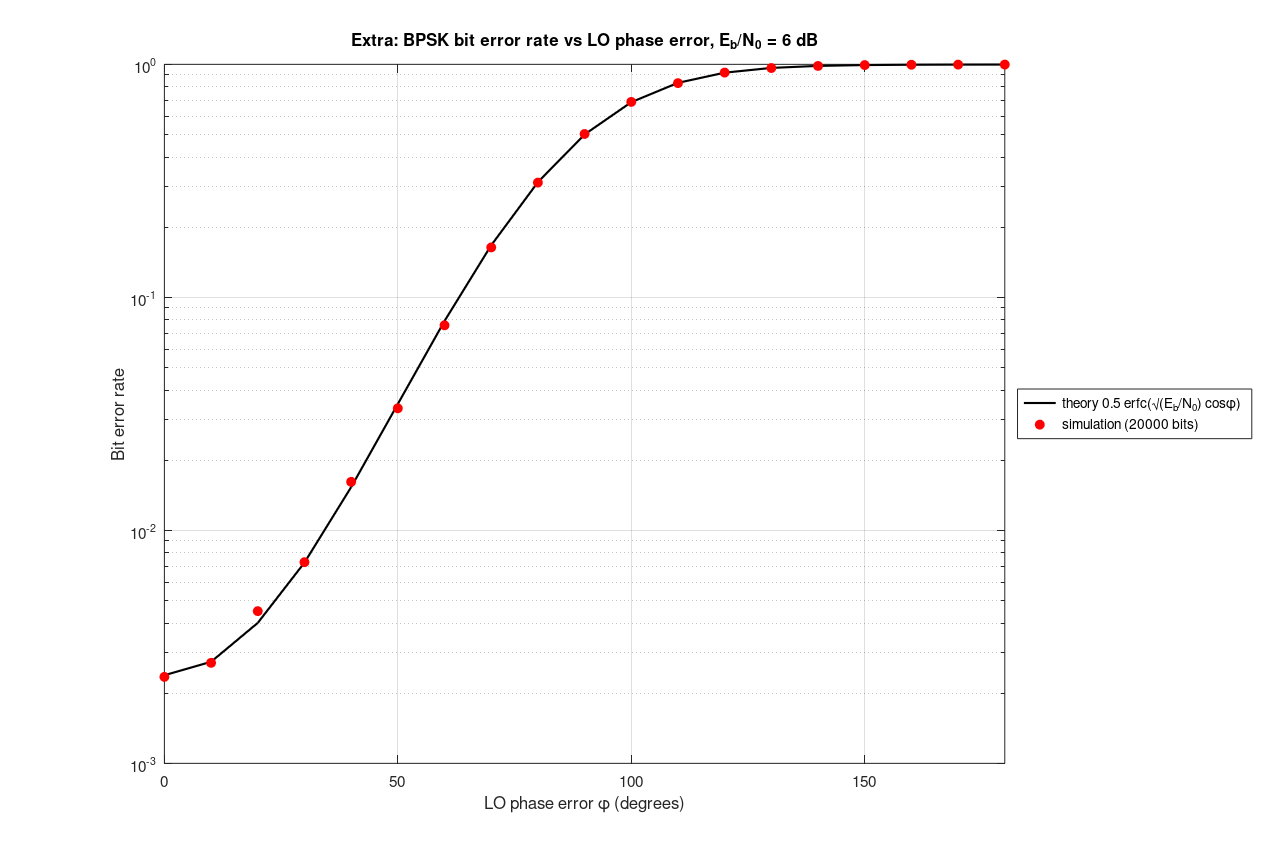
\includegraphics[width=0.85\textwidth]{Octave Scripts/digB_2_figures/05_extra_ber_vs_phase.png}
  \caption{Extra: BPSK bit error rate against LO phase error at $E_b/N_0 = 6$ dB, simulation (20000 bits) overlaid on theory.}
\end{figure}

\medskip
\noindent\textbf{e.} \textit{Effect of the line code.} We replaced the polar NRZ waveform by the AMI waveform of Item~1 (marks alternate between $+1$ and $-1$ in half-width pulses, spaces are $0$) as the modulating signal. The modulator is a product, so the transmitted PSD is simply the PSD of the line code translated to $\pm f_c$. For AMI, $S_{\text{AMI}}(f) = \frac{A^2 T_b}{4}\operatorname{sinc}^2(fT_b/2)\sin^2(\pi f T_b)$, and the modulated PSD is $\frac{1}{4}\left[S_{\text{AMI}}(f - f_c) + S_{\text{AMI}}(f + f_c)\right]$. The line code therefore changes the transmitted spectrum in four ways:
\begin{itemize}
  \item \textbf{Notch at the carrier.} AMI has no power at DC, so the modulated signal has a notch at $f_c$ with two lobes peaking near $f_c \pm 0.5R_b$, while the BPSK of polar NRZ has its maximum at $f_c$.
  \item \textbf{Same null-to-null width.} The first nulls are still at $f_c \pm R_b$, so the main lobe still spans $2R_b = 2$ Hz.
  \item \textbf{Less power.} For the same pulse amplitude the average transmitted power drops from $0.500$ V$^2$ to $0.128$ V$^2$ (theory $0.125$ V$^2$), because only half of the bits are marks and each mark fills only half of the bit.
  \item \textbf{Wider 1\% bandwidth.} It grows from $77.0$ Hz to $137.3$ Hz (theory curve $134.8$ Hz): the sidelobe tails of the two signals are similar, but the AMI peak is about 7 dB lower, so the same tails are a larger fraction of the maximum.
\end{itemize}
The signal also loses its constant envelope: it takes three amplitude levels ($0$ and $\pm 1$), which needs a linear amplifier. The receiver still works: after the same mixer, integrating over the first half of every bit decodes the AMI stream with \textbf{0 errors}.

\begin{figure}[H]
  \centering
  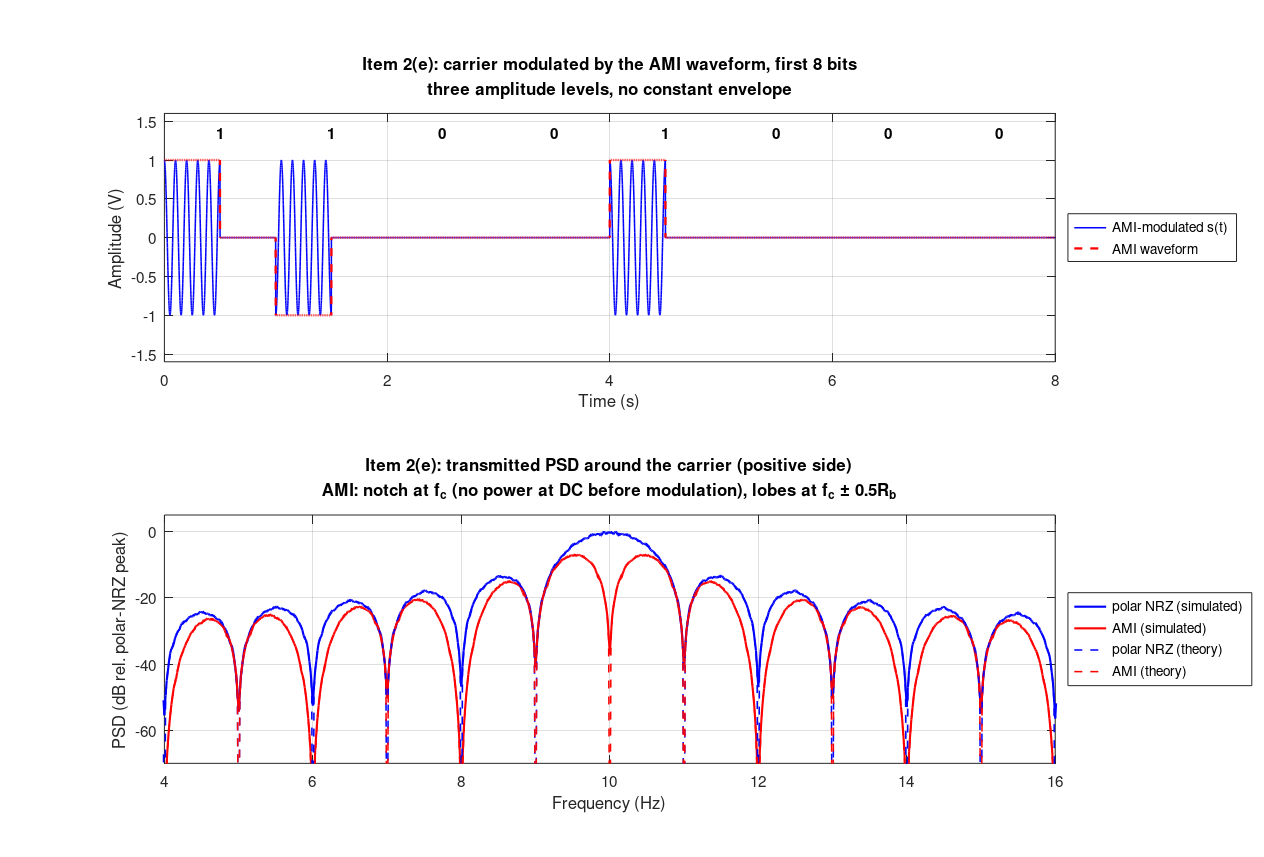
\includegraphics[width=0.95\textwidth]{Octave Scripts/digB_2_figures/04_item2e_linecode.png}
  \caption{Item 2(e): carrier modulated by the AMI waveform, first 8 bits (top), and transmitted PSD around the carrier for polar NRZ and AMI, simulation overlaid on theory (bottom).}
\end{figure}

\begin{table}[H]
\centering
\caption{Numerical results for Digital Part B, Item 2 (BPSK, $R_b = 1$ bit/s, $f_c = 10$ Hz)}
\begin{tabular}{l c}
\toprule
\textbf{Parameter / Metric} & \textbf{Value} \\
\midrule
Null-to-null bandwidth, polar NRZ BPSK & $2.00$ Hz ($=2R_b$) \\
1\% bandwidth, polar NRZ BPSK (simulated / theory curve) & $77.0$ Hz / $75.1$ Hz \\
1\% bandwidth, AMI-modulated carrier (simulated / theory curve) & $137.3$ Hz / $134.8$ Hz \\
Average power, polar NRZ BPSK / AMI-modulated carrier & $0.500$ V$^2$ / $0.128$ V$^2$ \\
Bit errors, $\phi = 0^\circ$ / $30^\circ$ / $60^\circ$ / $90^\circ$ (64 bits, no noise) & 0 / 0 / 0 / 31 \\
Detected amplitude, $\phi = 30^\circ$ / $60^\circ$ / $90^\circ$ (relative to $\phi = 0^\circ$) & $0.866$ / $0.500$ / $0$ \\
Bit errors, AMI-modulated carrier (64 bits, no noise) & 0 \\
\bottomrule
\end{tabular}
\end{table}
 \subsection{Part C: End-to-End System Integration}
  
    In this part, we assemble the individual functional blocks developed in Part~A and Part~B into a       
    unified end-to-end communication system:
    \begin{equation*}
    m(t) \;\xrightarrow{\text{sample}}\; m[k] \;\xrightarrow{\text{quantize}}\; m_q[k]
    \;\xrightarrow{\text{PCM encode}}\; b[n] \;\xrightarrow{\text{line code}}\; x_{\text{NRZ}}(t)          
    \;\xrightarrow{\text{BPSK mod}}\; s(t) \;\xrightarrow{\text{coherent det}}\; \hat{b}[n]
    \;\xrightarrow{\text{decode}}\; \hat{m}_q[k] \;\xrightarrow{\text{ideal LPF}}\; \hat{m}(t)             
    \end{equation*}
  
    \paragraph{1. Complete Transmitted Waveform Generation.}
    Following Part~A, the continuous-time analog message is:
    \begin{equation}
    m(t) = \cos(2\pi \cdot 20 \cdot t) + 0.5 \cos(2\pi \cdot 50 \cdot t), \quad W = 50\text{ Hz}
    \end{equation}
    The message is sampled at $f_s = 400\text{ Hz} = 4 f_{\text{Nyquist}}$, producing $N_s = 400$ samples 
    over $T = 1\text{ s}$. As determined in Part~A Item~4(d), achieving an $\text{SQNR} \ge 40\text{ dB}$  
    requires $n = 7\text{ bits}$ per sample ($L = 2^7 = 128$ levels). Using a mid-tread uniform quantizer 
    over the dynamic range $[V_{\min}, V_{\max}] = [-1.3529\text{ V}, +1.5000\text{ V}]$, the quantization
    step size is: 
    \begin{equation}
    \Delta = \frac{V_{\max} - V_{\min}}{L - 1} = \frac{2.8529}{127} \approx 0.02246\text{ V}
    \end{equation} 
    The quantized samples are serialized by the PCM encoder into an $N_b = 2800\text{ bit}$ stream at a bit
    rate $R_b = n \cdot f_s = 2800\text{ bits/s}$ ($T_b \approx 0.357\text{ ms}$). The bits are mapped to a
    polar NRZ line code ($\pm 1\text{ V}$) and modulated onto a sinusoidal carrier at $f_c = 14\text{ kHz} 
    > R_b$ using Binary Phase Shift Keying (BPSK): 
    \begin{equation}
    s(t) = x_{\text{NRZ}}(t)\cos(2\pi f_c t)
    \end{equation} 
    Figure~\ref{fig:digC_tx} shows the waveforms across the transmitter blocks.
  
    \begin{figure}[H] 
      \centering 
      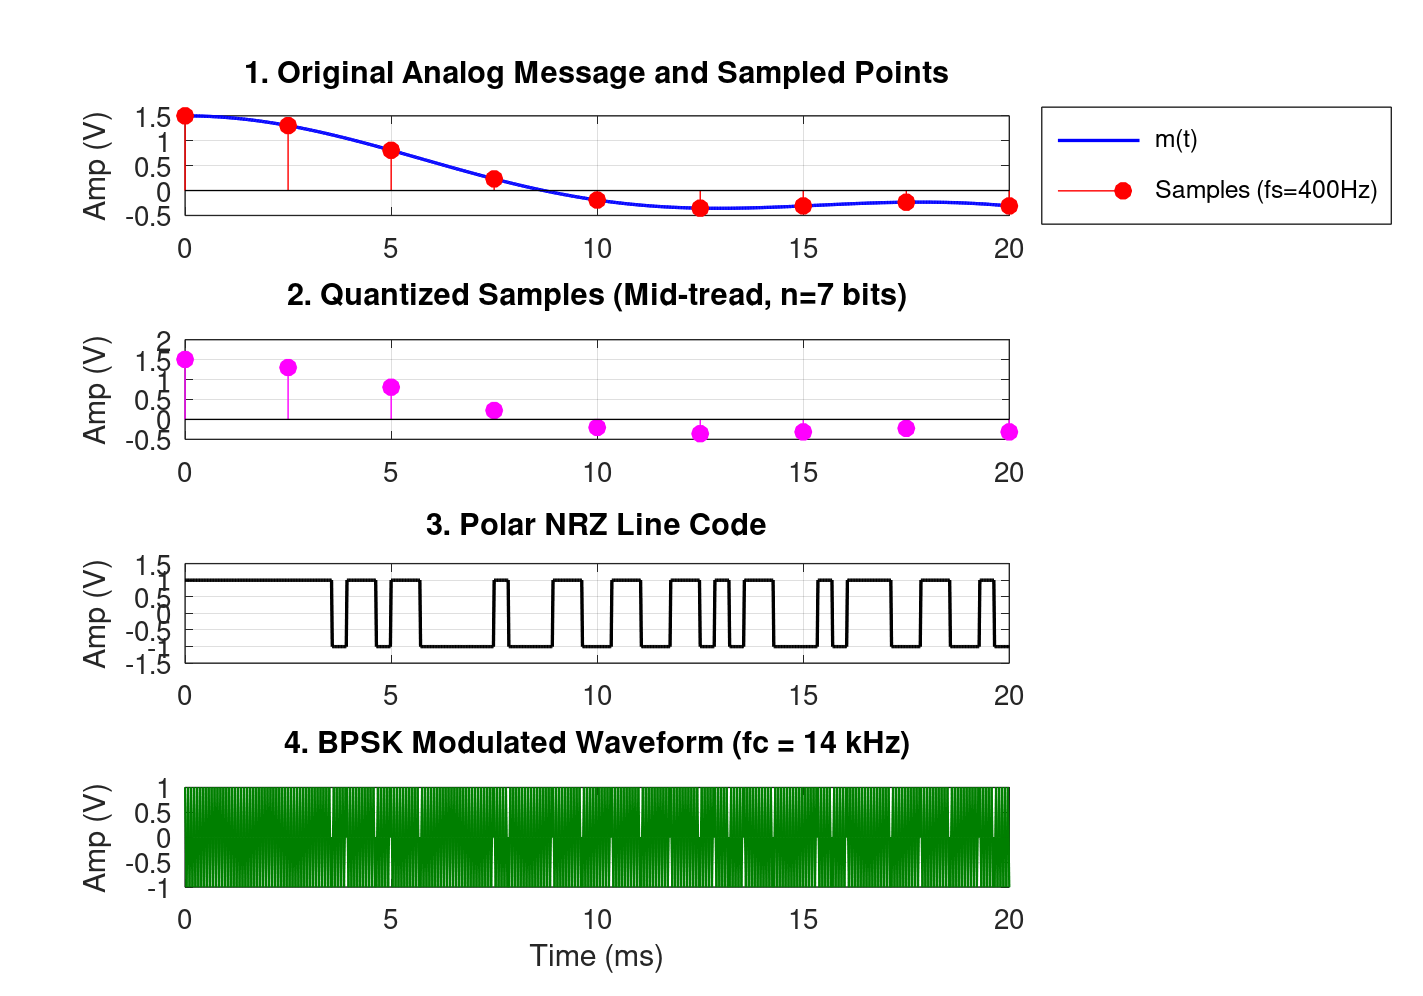
\includegraphics[width=0.95\textwidth]{Octave Scripts/digC_figures/01_tx_blocks_waveform.png} 
      \caption{Signal waveforms at the output of each transmitter block over the first 20~ms.}
      \label{fig:digC_tx}
    \end{figure}
  
    \paragraph{2. Coherent Detection and Bit Recovery.} 
    The coherent BPSK receiver mixes the incoming signal with a synchronized local carrier $2\cos(2\pi f_c
    t)$ and detects bit values using integrate-and-dump decision over each bit interval $[k T_b,       
    (k+1)T_b]$:
    \begin{equation}
    y[k] = \frac{1}{T_b}\int_{k T_b}^{(k+1)T_b} s(t) \cdot 2\cos(2\pi f_c t) \, dt = x_{\text{NRZ}}[k] +   
    \underbrace{\frac{1}{T_b}\int_{k T_b}^{(k+1)T_b} x_{\text{NRZ}}(t)\cos(4\pi f_c t)\,dt}_{\approx 0}    
    \end{equation}                                                                                         
    Because the channel is ideal and the local oscillator is phase-synchronized ($\phi = 0^\circ$), the    
    receiver recovers the bit stream with:                                                                 
    \begin{equation*}                                                                                      
    \textbf{Total Bit Errors} = 0 \quad (\text{out of } 2800\text{ bits})                                  
    \end{equation*}                                                                                        
    Figure~\ref{fig:digC_rx} confirms the exact match between the transmitted and received bits. If bit    
    errors were observed, they could arise from local oscillator phase offset $\phi$ (degrading detection  
    margin by $\cos\phi$), timing jitter at the decision slicer, channel band-limiting (intersymbol        
    interference), or additive noise.                                                                      
                                                                                                           
    \begin{figure}[H]                                                                                      
      \centering                                                                                           
      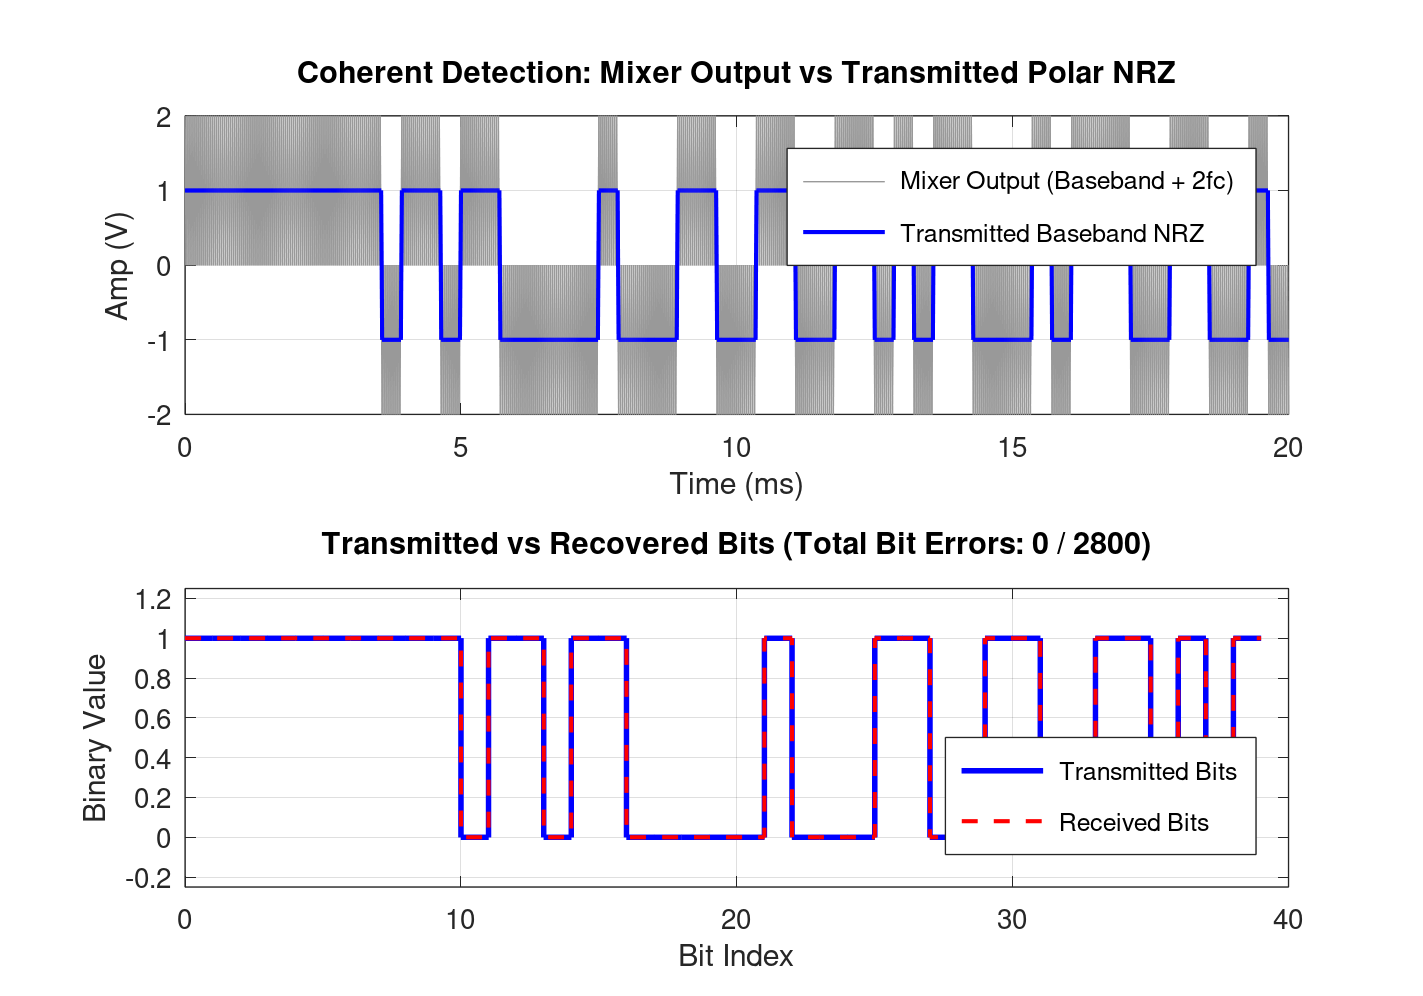
\includegraphics[width=0.95\textwidth]{Octave Scripts/digC_figures/02_rx_bit_recovery.png}           
      \caption{Coherent demodulation (top) and comparison of transmitted vs.\ received bit stream          
      (bottom).}                                                                                           
      \label{fig:digC_rx}                                                                                  
    \end{figure}                                                                                           
                                                                                                           
    \paragraph{3 \& 4. Analog Reconstruction and Error Analysis.}                                          
    The recovered bit stream is demultiplexed into 7-bit codewords, translated to level indices, and       
    converted to discrete-time quantized levels $\hat{m}_q[k]$. The analog message is reconstructed by     
    passing the weighted impulse train through an ideal low-pass filter with cutoff $f_{\text{cut}} = W =  
    50\text{ Hz}$ and passband gain $T_s$.                                                                 
                                                                                                           
    Figure~\ref{fig:digC_recon} illustrates the reconstructed signal $\hat{m}(t)$ plotted together with the
    original message $m(t)$, as well as the point-by-point reconstruction error $e(t) = m(t) - \hat{m}(t)$.
                                                                                                           
    \begin{figure}[H]                                                                                      
      \centering                                                                                           
      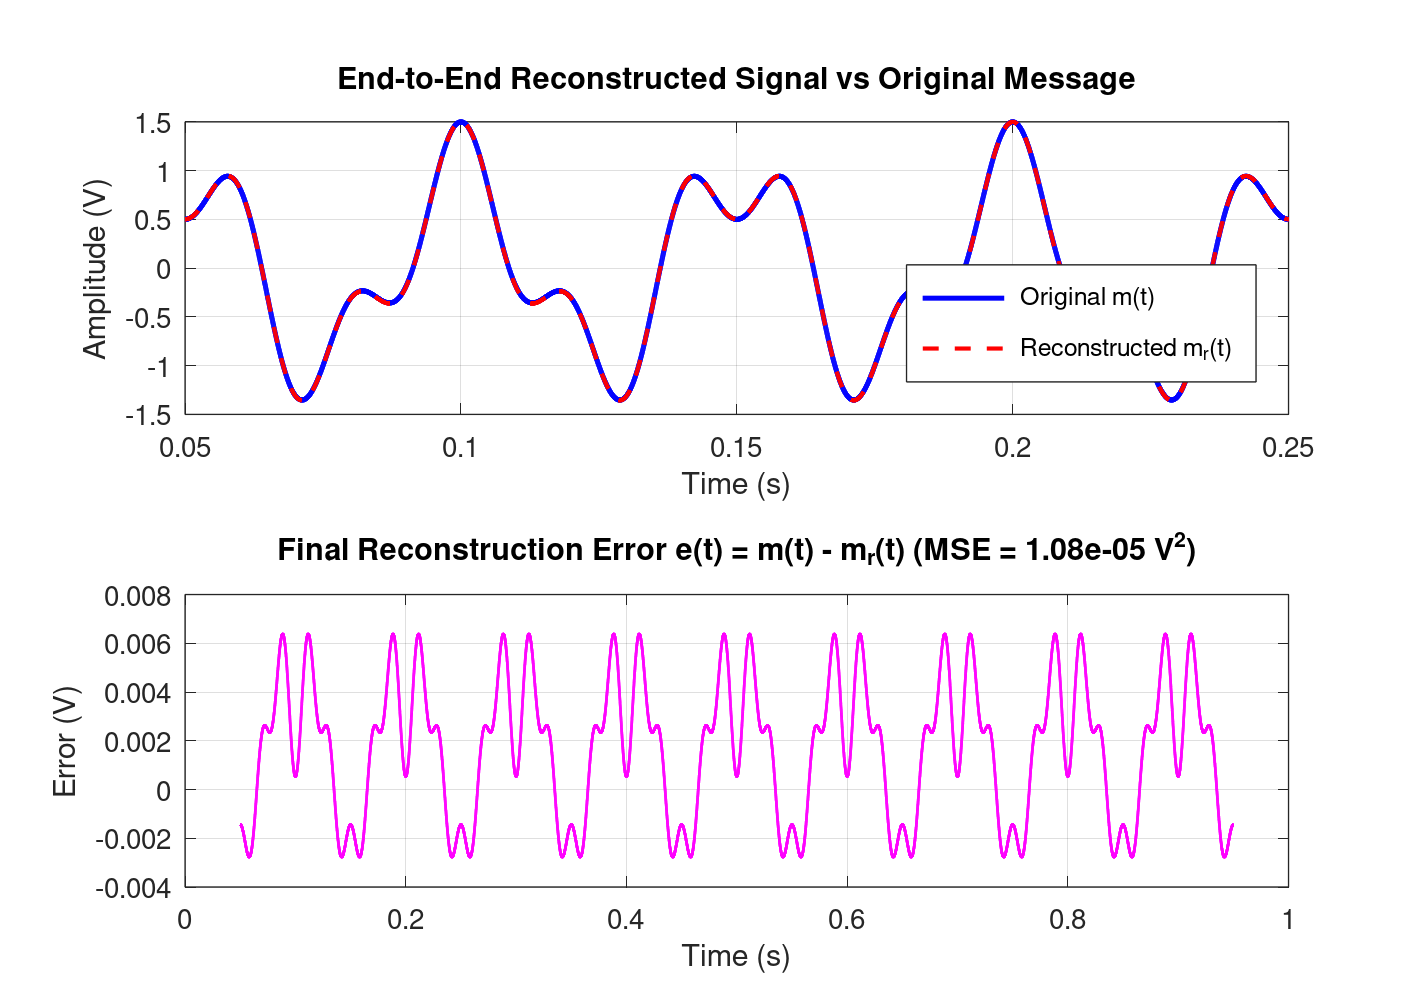
\includegraphics[width=0.95\textwidth]{Octave Scripts/digC_figures/03_reconstruction_and_error.png}  
      \caption{Top: Reconstructed analog signal $\hat{m}(t)$ overlaid on original $m(t)$. Bottom: Total    
      reconstruction error $e(t)$.}                                                                        
      \label{fig:digC_recon}                                                                               
    \end{figure}                                                                                           
                                                                                                           
    \begin{figure}[H]                                                                                      
      \centering                                                                                           
      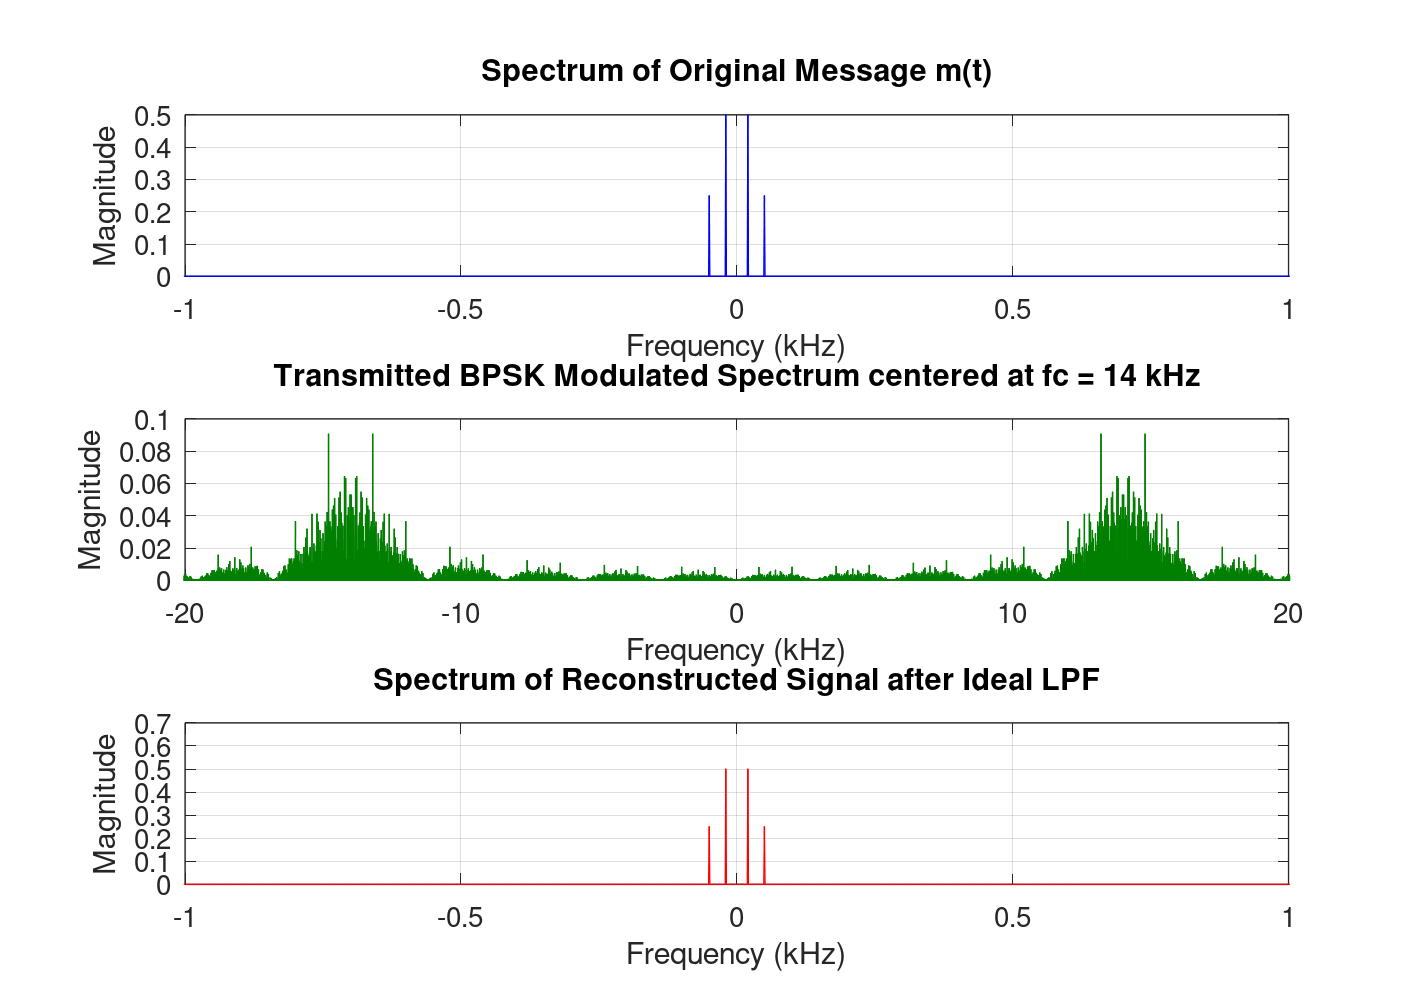
\includegraphics[width=0.95\textwidth]{Octave Scripts/digC_figures/04_system_spectra.png}            
      \caption{Magnitude spectra across the system: baseband message (top), transmitted BPSK signal        
      (middle), and recovered reconstructed spectrum (bottom).}                                            
      \label{fig:digC_spectra}                                                                             
    \end{figure}                                                                                           
                                                                                                           
    \paragraph{Measurement and Source of Error.}                                                           
    The numerical error metrics obtained from the simulation are:                                          
    \begin{itemize}                                                                                        
      \item \textbf{Quantization MSE ($e_q^2$):} $4.18\times 10^{-5}\text{ V}^2$ ($\text{SQNR} \approx     
      41.75\text{ dB}$).                                                                                   
      \item \textbf{Total Reconstruction MSE ($e_r^2$):} $4.21\times 10^{-5}\text{ V}^2$ ($\text{SQNR}     
      \approx 41.72\text{ dB}$).                                                                           
    \end{itemize}                                                                                          
    The reconstruction error is dominated by the **quantization error** inherent in representing continuous
    amplitudes with $n = 7$ bits ($128$ levels). The slight discrepancy between reconstruction MSE and     
    quantization MSE stems from the finite observation window ($T = 1\text{ s}$), where truncation of the  
    ideal low-pass filter sinc interpolation tails introduces mild edge ringing (Gibbs phenomenon).        
                                                                                                           
    \paragraph{Could the error be made smaller?}                                                           
    Yes:                                                                                                   
    \begin{enumerate}                                                                                      
      \item \textbf{Increase bit resolution $n$:} Each additional bit increases the SQNR by approximately  
      $6.02\text{ dB}$, decreasing the MSE by a factor of 4.                                               
      \item \textbf{Non-uniform quantization ($\mu$-law / $A$-law):} Concentrates quantization steps where 
      message probability density is highest.                                                              
      \item \textbf{Filter windowing:} Applying windowed sinc interpolation or raised-cosine smoothing to  
      eliminate finite-duration boundary transients.                                                       
    \end{enumerate}                                                                                        
                                                                                                           
    \paragraph{5. Fault Diagnosis Check.}                                                                  
    Because the total reconstruction error closely matches the theoretical quantization error              
    ($\text{MSE}_{\text{recon}} \approx \text{MSE}_{\text{quant}}$) and the bit error count is strictly    
    zero, no intermediate stage (carrier modulation, demodulation, PCM decoding) introduced degradation.


\end{document}
